\chapter{Spectral Neural Representation of Seamless Textures}
\label{chap:seamless-textures}

Textures play a fundamental role in computer graphics, providing essential information about material properties, surface characteristics, and spatial variations. These elements enhance the visual complexity of virtual environments, allowing for the representation of intricate patterns and micro-scale details that are otherwise difficult to model procedurally. Among these, \textit{periodic textures} are particularly significant, characterized by repeating patterns that exhibit regularity along one or more spatial dimensions. Such textures are frequently employed to model materials in domains like architecture, textiles, and industrial design, where repetitive structures are common. Capturing the properties of periodic textures effectively is an important task for achieving realistic visual representations in virtual scenes.

In traditional approaches, textures are typically represented as discrete digital tiles, often accompanied by methods to mitigate visible seams or discontinuities when textures repeat. In contrast, we propose to use our multiresolution neural representation to encode seamless periodic textures in a continuous, compact and fast to evaluate digital representation. Specifically, we extend deep sinusoidal neural networks to define \textit{periodic neural networks}. Inspired by the Fourier series, we constrain the representational space of our network to the space of periodic functions.

A key theoretical contribution of this work is demonstrating that if the first layer of a sinusoidal neural network is initialized with frequencies that are integer multiples of a period $P$, then the resulting network exhibits periodicity with the same period $P$. This is a consequence of the fact that the composition of sinusoidal layers expands as a sum of sines with frequencies given by integer combinations of the input layer, and the result is similarly periodic~\citep{novello2022understanding, yuce2022structured}. effectively encodes periodic textures and can be used to generate seamless versions of these textures. Furthermore, it can be seamlessly integrated into existing graphics pipelines for texture mapping applications.

Periodic networks allows us to represent a periodic texture in a infinite domain by training it only in a small tile. For non-tileable data, we introduce a regularization term based on the \textit{Poisson equation} to enforce that the image produced by a periodic network forms a seamless, tileable texture -- meaning it should tile across the plane without displaying noticeable seams or discontinuities at the tile boundary. 

Additionally, based on Fourier series, we propose a frequency initialization strategy that significantly reduces the number of possible choices for frequencies. Besides the periodic representation, our method leads to better representation quality of periodic images, using fewer parameters in the network architecture. Moreover, it can be applied to non-periodic signals by periodicizing them through repetition or reflection. Once trained, the network can accurately reconstruct the original signal by evaluating only within the training domain.

% Specifically, we enforce the gradient of the network within the tile domain to match the gradient of the original texture (Poisson constraint), while 

% One of the main advantages of periodic neural networks is their ability to represent textures over an infinite domain by training on a single texture tile. This reduces the need for extensive datasets or repetitive training. For non-tileable textures, we introduce a regularization term based on the \textit{Poisson equation}, which enforces the seamless property. 

% The key idea is to enforce the INR gradient of the network to match the original gradient within the domain (Poisson equation) and to ask the INR to be equal to an image average on the domain border (periodic boundary values)~\cite{perez2003}. It is important to note that for this problem to be well-posed, the boundary must be closed. However, since our network is periodic, we are solving the Poisson problem on the torus which allows us to also require gradient matching on the domain boundary (see the results in Section \ref{s:poisson-regularization}).






% %%%%%%%%%%%%%%%%%%%%%%%%%%%%%%%%%%%%%%%%%%%%%%%%%%%%%%%%%%%%%%%%%%%%%%%%%%%%%%%%%%%%%%%
\section{Related Works}

% The scope of this chapter is to represent seamless material textures using \textit{implicit neural representations} (INRs). Thus, it aims to encode the material texture of a surface through a periodic neural network $f_\theta:\mathbb{R}^2\to \mathcal{C}$, where $\mathcal{C}$ is a color space such as grayscale or \texttt{RGB}, and $\theta$ is the set of parameters of the network that can be trained based on data samples. More generally, this representation could be extended to the other channels of a material definition such as the specular or normal channels.

% In this sense, the context is texture creation methods (procedural-based, capture-based, AI-based, and manual) with the purpose of being applied to a 3D surface by a rendering system.

% Generating high-quality textured materials is challenging as they need to be visually realistic, seamlessly tileable, and have a small impact on the memory consumption of the application. For this reason, these materials are often created manually by skilled artists. In this chapter, we show that INRs can be used in those tasks.

% Additionally, it is desirable to have an agnostic material representation based on industry standards that is compatible with most rendering systems. One case is the Substance 3D Sampler from~\citet{substance_sampler}, a creation platform of material collections that includes many tools for that very purpose. Next, we discuss the most relevant works that are related to our method.

Generating high-quality textured materials is a longstanding challenge in computer graphics, requiring them to be visually realistic, seamlessly tileable, and efficient in memory usage. To meet the demands of compatibility with standard industry pipelines, it is desirable to have a material representation that is agnostic to specific rendering systems. One example of this is the Substance 3D Sampler by \citet{substance_sampler}, a widely used platform for creating material collections with various tools to achieve realistic results. Below, we review relevant works that connect to our method, particularly in the context of periodic texture synthesis and representation.

% Traditionally, skilled artists create these materials manually to ensure high fidelity and performance. In this chapter, we demonstrate that Implicit Neural Representations (INRs) can be effectively used for such tasks, offering an automated, compact, and continuous representation of textures.

% \subsection{Texture representations}

% Textures are a foundational component in computer graphics, critical for synthesizing realistic surfaces and patterns based on photographic exemplars. 
Texture synthesis has evolved into a mature field with a wide array of methods, including classic texture mapping~\citep{blinn76}, procedural textures~\citep{perlin-1985}, synthesis-by-example~\citep{efros99}, and user-guided texture generation~\citep{haeberli90}. \citet{pauly-2009} offers an extensive overview of example-based texture synthesis methods, while \citet{etal-2010} provides a detailed account of noise primitives for procedural texturing. More recently, \citet{rethinkngtex} discuss alternative methods for texture mapping, particularly in the context of overcoming traditional limitations.
%
% Recently, \citet{rethinkngtex} discusses alternative texture-mapping methods. Most of the these previous methods target general texture patterns. However, there is a trend that investigates models of specific materials. This approach has the benefit of producing higher fidelity results by exploiting characteristics of important materials, such as wood. \citet{dorsey-2004} studies aggregate materials that are common in nature and formed by small particles.

Although many of these techniques focus on general texture patterns, there has been a growing interest in models tailored for specific materials. Such approaches provide higher fidelity by leveraging the unique properties of materials like wood, stone, or fabric. For instance, \citet{dorsey-2004} investigates aggregate materials formed by small particles, which are common in nature. These material-specific methods allow for more precise control, yet they often lack generalization across various domains.

% \subsection{Tileable Textures}

While there is a large body of research devoted to texture mapping, little work has been dedicated to synthesizing seamless tileable textures, which are important for the creation of materials. These textures have the property that when laid out in a regular grid of tiles they form a homogeneous appearance suitable for use in memory-sensitive real-time graphics. \citet{tileinteractive} gives an overview of tile-based methods in computer graphics applications.


% real-time graphics applications where memory is limited. 
Despite significant advancements in texture mapping, relatively little research has focused on synthesizing seamless, tileable textures, which are important for the creation of materials. Tileable textures enable the creation of homogeneous surfaces by repeating a small tile across a plane without visible seams. \citet{tileinteractive} reviews tile-based methods in this context, while \citet{tilehard} presents an algorithm for generating non-periodic virtual textures from a small set of stored tiles. \citet{Moritz2017Texture} introduces an approach to synthesizing tileable textures using the PatchMatch algorithm. However, these methods rely on specialized algorithms that must be integrated into the rendering pipeline. In contrast, our approach leverages neural networks to represent tileable textures that can be exported or evaluated directly on the graphics hardware, providing a more general and flexible solution.
%
% Additionally, we highlight the following methods. \citet{tilehard} presents a tile-based texture mapping algorithm that generates an arbitrarily large and non-periodic virtual texture map from the small set of stored texture tiles. \citet{Moritz2017Texture} developed an approach to synthesize tileable textures using the PatchMatch texture synthesis algorithm. These methods rely on a particular algorithm that must be incorporated into the rendering system. Our INR representation, once trained is exported to be evaluated on the graphics hardware or, alternatively, can be used to generate a material tile.

A notable contribution to the creation of seamless texture from a single tile comes from \citet{perez2003}, who proposed making a texture tileable by solving a Poisson problem, ensuring that opposite sides of a rectangular domain match. Their method enforces gradient consistency within the texture while equating opposite boundaries. However, this approach is limited to raster-based representations. Our method incorporates a regularization term for training periodic neural representation to produce seamless texture. By solving the Poisson equation on the 2D torus, we can interchange the boundary and interior equations.

% \subsection{Neural Textures}

Texture representations aim to integrate procedural techniques with data sample fitting. The primary trade-off lies between computational efficiency and memory usage. Promising solutions to this challenge are offered by \emph{wavelets} and \emph{neural networks}. For instance, \citet{BAJAJ-2000} tackled the memory issue by employing a wavelet-based method to encode 3D textures. Meanwhile, \citet{Gutierrez-2019} introduced a generative deep learning framework for 3D texture synthesis based on style transfer. Their results are comparable to those of patch-based approaches.

Several works aim to integrate procedural techniques with data-driven approaches to achieve a balance between computational efficiency and memory usage. Neural networks are promising in this regard. For instance, \citet{Gutierrez-2019} applied a deep learning framework for 3D texture synthesis using style transfer, achieving results comparable to patch-based methods. For tileable textures specifically, \citet{deeptile} introduced a deep learning method for synthesizing example-based textures at arbitrary resolutions. Similarly, \citet{zhou2022tilegen} used a modified StyleGAN to generate periodic material maps. While these methods rely on large datasets and generative models, our approach is fundamentally different: we employ coordinate-based neural networks in a spectral domain, achieving compact, data-efficient representations without requiring extensive training datasets. This distinction allows us to train faster and fit within resource-constrained applications.

% , making our method highly suitable for real-time rendering scenarios.


% However, these approaches still rely on extensive datasets and cannot leverage the compact, coordinate-based representation that we propose.

% Wavelet-based techniques~\citep{BAJAJ-2000} and  

% For tileable textures, \citet{deeptile} introduced an example-based texture synthesis approach using deep learning. This method creates tiles at arbitrary resolutions that closely resemble the structural components of an input texture. Similarly, \citet{zhou2022tilegen} devised a variant of StyleGAN with modifications to generate periodic material maps. While these studies utilize "data-based neural networks" and generative models, our approach employs "coordinate-based neural networks" and a spectral representational model. Our goal is to have a compact and fast to train representation that does not depend on training in a large dataset.

Alternatively, \citet{ntc2023} proposed a neural compression technique tailored to material textures, while \citet{match} introduced a deep learning method for constructing procedural materials based on neural features. \red{MELHORAR...In this context, our model offers a compact solution that can seamlessly integrate into a neural rendering pipeline.}

% \subsection{Implicit neural representations}

BACON \citep{bacon2021} is analyticaly equivalent to a shallow network, so it is clear that the representation can be made periodic by initializing the first layer with frequencies that are integer multiples of a period $P$. However, for deep sinusoidal MLP such as Siren \cite{sitzmann2019siren} or MR-Net, this could not be true, since the composition of sines can generate much more frequencies. Figure \ref{f:generated-frequencies} shows the magnitude of frequencies, computed using the Fast Fourier transform (FFT), for signals generated by the sum of sines, product of sines, product of a sine by a sum of sines, and composition of sines. It is evident that the composition of sines produces a larger number of frequencies compared to the other options.

% builds upon \textit{Multiplicative filter networks} (MFNs) \cite{fathony2020multiplicative} to control frequencies in the network and represent signals at multiple scales. As this representation is analyticaly equivalent to a shallow network, it is clear that the representation can be made periodic by initializing the first layer with frequencies that are integer multiples of a period $P$. 

% One of the most relevant works to our method is Bacon~\citep{bacon2021}, which builds on \emph{Multiplicative Filter Networks} (MFNs)~\citep{fathony2020multiplicative} to control frequencies at multiple scales. While Bacon's representation can be made periodic by initializing the first layer with integer multiples of a period $P$, this holds true primarily for shallow networks. For deeper networks, like our sinusoidal MLPs (Siren or MR-Net), the composition of sine layers generates a wider range of frequencies. As illustrated in Figure~\ref{f:generated-frequencies}, which shows the frequency magnitude from the Fourier transform of different combinations of sinusoidal functions, deeper architectures significantly expand the frequency space, resulting in a richer set of periodic representations.

\begin{figure}[h]
\centering
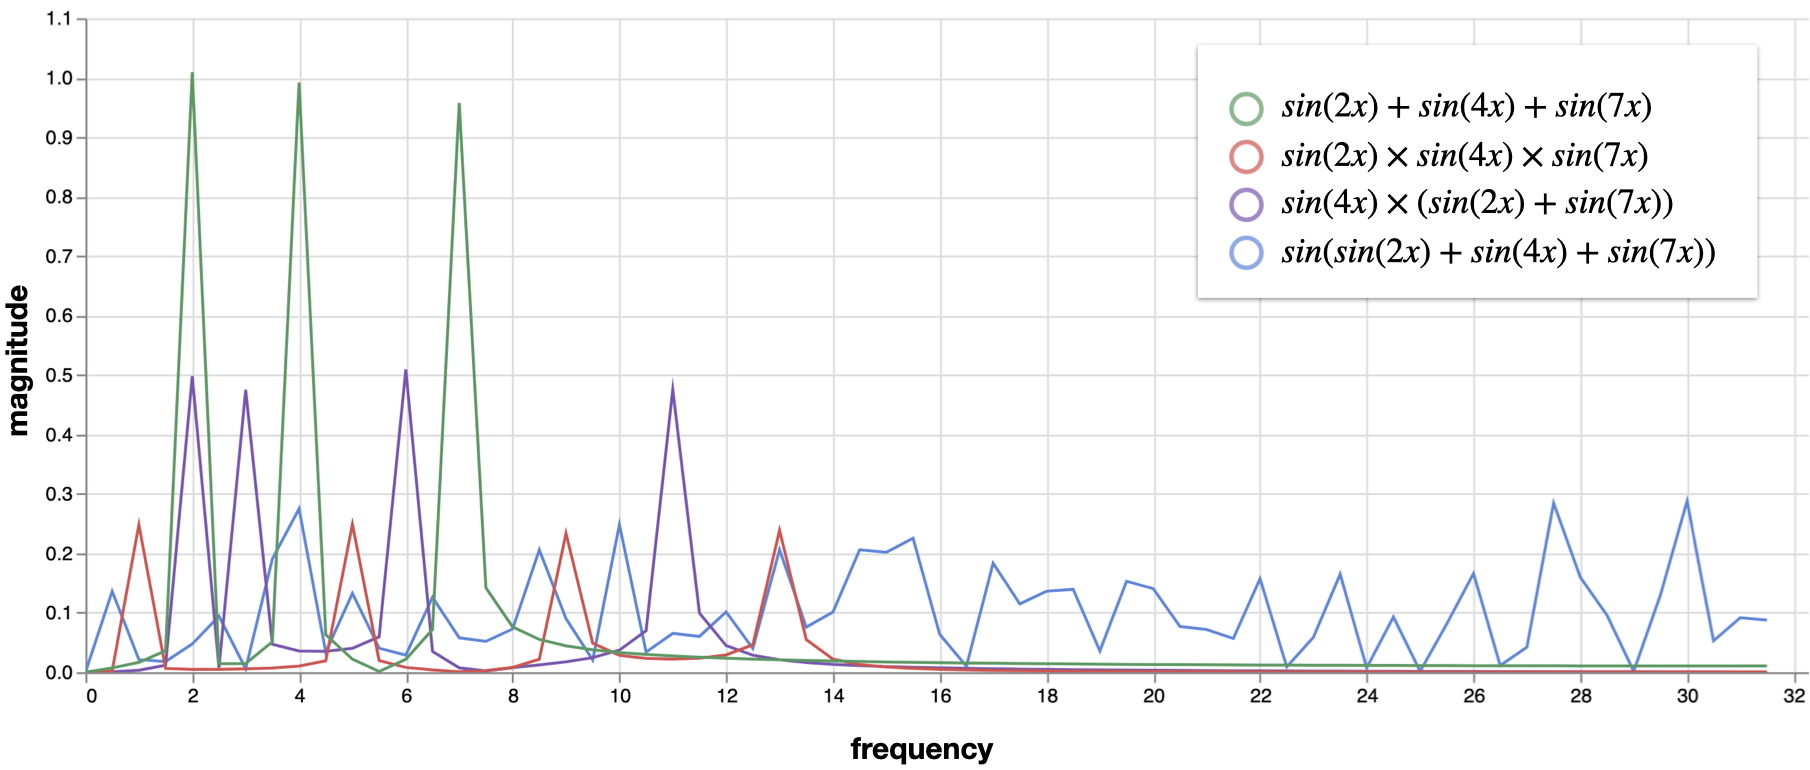
\includegraphics[width=0.80\linewidth]{img/ch6/generated_frequencies.png}
\caption{Fourier Transform of different combinations of sinusoidal functions.}
\label{f:generated-frequencies}
\end{figure}
    
% Regarding seamless textures, inspired by~\cite{perez2003}, we model it as a term in the loss function using a Poisson problem. This strategy has been explored in INRs for tasks such as compositing gradients~\cite{sitzmann2019siren, schardong2024neural}. SIREN trains the INR using only the gradients, leading to the learning of the signal up to an integral constant, which is problematic when we have multiple channels. In contrast, our training scheme incorporates both gradient and image values.

Finally, our seamless texture generation draws inspiration from \citet{perez2003}, where Poisson problems were used to enforce tileability in pixel-based images. This strategy has been extended in INR-based methods for gradient compositing~\citep{sitzmann2019siren, schardong2024neural}. While SIREN optimizes for gradient fields only, potentially leaving integral constants ambiguous, our training framework incorporates both image values and gradients, ensuring a more robust fit across multiple channels and yielding higher-quality seamless textures.


% % %%%%%%%%%%%%%%%%%%%%%%%%%%%%%%%%%%%%%%%%%%%%%%%%%%%%%%%%%%%%%%%%%%%%%%%%%%%%%%%%%%%%%%%
\section{Periodic Neural Networks}

Throughout this section, we assume that the signal is a monochromatic image, though the results can easily extend to multi-channel images or any signal with an explicit representation in its natural domain as a function \( \gt{f}: \mathbb{R}^n \to \mathbb{R}^m \).

A \textit{periodic image} $\gt{f}:\mathbb{R}^2\to \mathbb{R}$ is a function satisfying the property $\gt{f}(x) \!=\! \gt{f}(x + P)$ with $P=(P_1, P_2)\in \mathbb{R}^2$ giving the \textit{periods} along the axes $x_1$ and $x_2$.
For instance, a \textit{harmonic function} $h(x_1, x_2)=a\sin(x_1\omega_1+x_2\omega_2+ \varphi)$ represents a simple periodic signal, where $\omega_i\!=\!k_i\frac{2\pi}{P_i}$, with \( k_i \in \mathbb{Z} \), are the \textit{frequencies}, $a$ is the \textit{amplitude}, and $\varphi$ is the \textit{phase shift}.
Harmonic functions like this play a central role in \textit{Fourier series}, where any periodic function $\gt{f}$ can be approximated by a sum of harmonic components.

We will show how sinusoidal neural networks can be transformed into periodic neural networks through the proper choice of the weights in the first sinusoidal layer.

% A **periodic image** \( f: \mathbb{R}^2 \to \mathbb{R} \) is defined as a function that satisfies the property \( f(x) = f(x + P) \), where \( P = (P_1, P_2) \in \mathbb{R}^2 \) are the periods along the axes \( x_1 \) and \( x_2 \). 
% For instance, a **harmonic** function \( h(x_1, x_2) = a \sin(x_1 \omega_1 + x_2 \omega_2 + \varphi) \) represents a simple periodic signal, where \( \omega_i = k_i \frac{2\pi}{P_i} \) with \( k_i \in \mathbb{Z} \) are the **frequencies**, \( a \) is the **amplitude**, and \( \varphi \) is the **phase shift**. 

% Harmonic functions like this play a central role in **Fourier series**, where any periodic function \( f \) can be approximated as a sum of harmonic components.


\subsection{Shallow Sinusoidal networks}

We observe that a shallow sinusoidal network $f:\R^2\to \R$, that is one with only a single sinusoidal layer, can be described as a sum of harmonic functions:

% Observe that summing harmonic functions also results in a \textit{sinusoidal network} $f:\R^2\to \R$ with a single layer:
\begin{align}\label{e-fourier_series}
    f(x) = L\circ s(x) =  c_0 + \sum_{i=1}^{n} c_i  \sin\Big(\dot{\omega_i}{ x}+ \varphi_i\Big)
\end{align}

where the \textit{first layer} $S:\R^2\to \R^{n}$ projects the input coordinates $x=(x_1,x_2)$ into a list of harmonics:

\begin{align}\label{e-firstlayer}
\displaystyle
    s(x)=\sin(\omega x +\varphi)=
    \left(
    \begin{array}{c}
        \sin\big(\dot{\omega_1}{x}+\varphi_1\big)\\
         {\vdots}\\
         \sin\big(\dot{\omega_{n}}{x}+\varphi_{n}\big)
    \end{array}
    \right).
\end{align}

where $\dot{\omega_i}{x}=\omega_{i1}x_1+\omega_{i2}x_2$. The matrix $(\omega_1, \ldots, \omega_{n})$ provides the \textit{frequencies}, and the bias vector $(\varphi_1, \ldots, \varphi_{n})$ gives the \textit{phase shifts}. The \textit{linear layer} $L$ combines the harmonics with the \textit{amplitudes} $c_i$ and adds a bias $c_0$.

For the network $f$ to be periodic with periods $(P_1,P_2)$ we can set the frequencies $\omega_{ij}=k_{ij}\frac{2\pi}{P_i}$, with $k_{ij}$ being integers. In Section~\ref{s-initialization}, we discuss a initialization strategy for choosing $k_{ij}$ using ideas from Fourier series.

\subsection{Deep sinusoidal networks}\label{s-deep-networks}

To create a deep sinusoidal neural network, we compose the first layer of $f$ with a hidden layer $H:\R^{n}\to \R^{m}$. Formally:
$f=L\circ H \circ \,S$, 

where $H\circ S(x):=\sin\big(W \cdot S(x)+b\big)$, with $W\in\R^{m\times n}$ as the \textit{hidden matrix}, and $b\in\R^{m}$ as the \textit{bias}.


The $i$th coordinate of $H$ can be expressed as a \textit{sinusoidal perceptron}:
%
\begin{align}
h_{i}\circ s(x)=\sin\left(\sum_{j=1}^{n} W_{ij} \sin\Big(\dot{\omega_j}{x}+\varphi_j\Big) + b_{i}\right).
\end{align}
%
Thus, $f$ consists of multiple sine compositions. Although  the activation function is periodic, the network $f$ may not keep this property. Even the sum of periodic functions can result in a non-periodic function: e.g. $\sin(x)+\sin\left(\sqrt{2}x\right)$. Furthermore, to accurately represent a periodic function, we must have control over the network's period.
% %
We observe that by initializing the first layer $s$ of a sinusoidal MLP $f$ with integer frequencies, specifically $\omega_{ij}=k_{ij}\frac{2\pi}{P_i}$ where $k_{ij}\in\Z$, we can prove that $f$ will be periodic with period $P=(P_1,P_{2})$.
In other words, $f(x_1, x_2)=f(x_1+P_1, x_2+P_2)$.

Without loss of generality, consider the case where $f$ is a 1D function, i.e. $f:\R\to\R$.%, the general case follows analogously. 
Assuming the first layer is periodic with period \( P \), its frequencies are \( \omega_j = k_j \frac{2\pi}{P} \).
\red{Moreover, observe that if we prove that if each sinusoidal neuron $h(x)=\sin\left(\sum_{i=1}^n a_j\sin(\omega_j x + \varphi_i)\right)$ expands as a sum of harmonics with period $P$, then, the output of $h$ is periodic with period $P$. The proof of this fact follows from} the following identity~\cite{novello2022understanding}:


\begin{align}\label{e-expansion}
    h(x)= \!\!\sum_{\textbf{l}\in\Z^n}\left[\prod_{i=1}^n J_{l_i}(a_i)\right]\sin\Big(\dot{\textbf{l}}{\omega x +\varphi}+ b\Big).
\end{align}

Since each frequency in this sum is written as $\dot{\textbf{l}}{\omega}=\frac{2\pi}{P}\dot{\textbf{l}}{\textbf{k}}$, we have that $h$ is periodic with period $P$.
We note that an expansion similar to Equation~\ref{e-expansion} was also presented in \cite{yuce2022structured}.

Another important fact to notice is that the amplitudes $\prod_{i=1}^n J_{l_i}(a_i)$ goes rapidly to zero as $\norm{\textbf{l}}_{\infty}$ increases. This is due to the following inequality~\cite{novello2022understanding}:
\begin{align}\label{e-upper-bound-freq}
    \abs{\prod_{i=1}^n J_{l_i}(a_i)}<
    \prod_{i=1}^n\frac{\left(\frac{\abs{a_i}}{2}\right)^{\norm{l_i}}}{\abs{l_i}!}.
\end{align}

For a sinusoidal MLP with two hidden layers, we use this conclusion to truncate the result given by the expansion of the first layer. This way, the input of the second hidden layer is a finite sum of sines and Equation~\ref{e-expansion} can be applied. By applying induction on this process, we conclude:

\begin{theorem}
\label{t-periodic}
    If the first layer of a sinusoidal MLP $f$ is periodic with period $P$, then $f$ is also periodic with period $P$.
\end{theorem}

Theorem~\ref{t-periodic} allows us to use sinusoidal MLPs to represent periodic functions. We define a \textbf{periodic neural network} as a sinusoidal MLP where the first layer is initialized to be periodic. Because MR-Net architectures are equivalent to progressively growing sinusoidal MLPs in width and depth, Theorem~\ref{t-periodic} also holds for MR-Net. Consequently, if we initialize each stage \( g_i \) of an MR-Net \( f: \mathbb{R}^n \times [0, N] \to \mathbb{R}^m \), \( f(x, t) = c_0(t) g_0(x) + \cdots + c_{N-1}(t) g_{N-1}(x) \), using integer frequencies, each level of detail within this representation maintains periodicity and the network remains periodic with respect to \( x \).

% Note that since MR-Net subclasses are analytically equivalent to a single sinusoidal MLP that can grow progressively in width and/or depth, if we initialize each stage $g_i$ of a MR-Net $f: \R^n \times \[ 0, N \] \to \R^m$, $f(x,t) = c_0(t)g_0(x) + \cdots + c_{N-1}(t)g_{N-1}(x)$ with integer frequencies, Theorem \ref{t-periodic} also applies and $f$ will be periodic with respect to $x$.

% In a more general sense, a \textit{sinusoidal network} is a function constructed by combining sinusoidal perceptrons.
% % %
% Furthermore, by adding more hidden layers to $f$, we obtain a sinusoidal \textit{multilayer perceptron} (MLP). Training such networks can be challenging because using the sine as an activation function may lead to instability in deep architectures~\cite{taming2017}. \citet{sitzmann2019siren} overcome this by proposing SIREN, which gives a special initialization scheme for sinusoidal MLPs, providing stability during training

% \subsection{Multiresolution sinusoidal networks}\label{s-mr-networks}
% \label{s-multiresolution}

% To represent textures using INRs we need to represent them in multiresolution. For this, we adopt the \textit{multiresolution network} (MRnet)~\cite{paz2022,paz2023mr} as a representation. Here, a MRnet is a network $f\!:\!\R^2\!\times\! [0,N]\!\to\! \R$ defined as a sum of $N$ periodic INR $g_i:\R^2\to\R$:
% \begin{align}
% f(x,t) = c_0(t)g_0(x) + \cdots + c_{N-1}(t)g_{N-1}(x),
% \end{align}
% The contribution of each \textit{stage} $g_i$ in Equation~\ref{e-mrnet} is controlled by $
% c_i(t)\!=\!\max\big\{0, \min\big\{1, t-i\big\}\big\}.$
% This allows us to navigate in the multiresolution using a parameter $t\!=\!k+\delta$ with $k\in\mathbb{N}$ and $0\leq\delta\leq 1$:
% \begin{align}\label{e-mrnet2}
% f(x,t)=g_0(x)+\dots + g_k(x)+\delta g_{k+1}(x).
% \end{align}

% The \textit{level of details} $f(\cdot, t)$ evolve continuously.
% We set the first layer of each periodic INR $g_i$ with integer frequencies, since Theorem~\ref{t-periodic} says that in this case $f$ will \textit{periodic} with respect to $x$.

% \section{Frequency initialization for Tilable Materials}
% \label{s-initialization}

% In this section, we introduce an initialization scheme for periodic neural networks based on a Fourier series interpretation. \red{This method ensures seamless tileable material representation by leveraging periodicity in the image approximation process.}

% Let $\gt{f}$ represent a ground-truth periodic image defined on a rectangular domain $[0, P_1] \times [0, P_2]$ with periods $(P_1, P_2)$. Our goal is to approximate $\gt{f}$ using an periodic neural network, denoted by $f$, that exhibits periodic behavior with the same periods $(P_1, P_2)$, ensuring seamless tiling. To achieve this, we define the weights $\omega_{ij}$ of the first layer of $f$ as $k_{ij}\frac{2\pi}{P_i}$, where $k_{ij}\in \mathbb{Z}^2$, thus ensuring the periodicity of the network as established by Theorem~\ref{t-periodic}.

% To define $k_{ij}$, we draw inspiration from Fourier series. According to the Fourier theorem, if $\gt{f} \in L^1(P)$, it can be represented as:

% \[
%     % \gt{f}(x) = \sum_{\textbf{k} \in \mathbb{Z}^2} c_{\textbf{k}} \, e^{i\dot{\omega}_{\textbf{k}} \cdot x},
%     \gt{f}(x)\!=\!\sum_{\textbf{k}\in \Z^2} c_\textbf{k} \text{e}^{i\dot{\omega_{{\textbf{k}}}}{ x}},
% \]

% where $c_{\textbf{k}}$ are the Fourier coefficients, and $\omega_{\textbf{k}} = 2\pi\left(\frac{k_1}{P_1}, \frac{k_2}{P_2}\right)$ with $\textbf{k} = (k_1, k_2)$. In practice, we truncate this series by summing over $\textbf{k} \in [-B, B]^2$, where $B$ is a bandlimit based on the frequencies in the ground truth signal. 

% \sloppy Since an input neuron can be rewritten as $\sin(\omega_i x + \varphi_i) = \cos(\varphi_i) \sin(\omega_i x) - \sin(\varphi_i)\sin\left(-\omega_i x + \frac{\pi}{2}\right)$, both $\omega_i$ and $-\omega_i$ are present in the signal. Therefore, we only need to sample the integer values $k_j$ from the half-square $\textbf{K} = [0, B] \times [-B, B]$ (Figure \ref{fig:1a}).

% The hidden layers are still initialized using the scheme from~\cite{sitzmann2019siren}. Although we initialize the first layer of $f$ with a finite and small number of frequencies from the set $\textbf{K}$, the composition of multiple layers results in the generation of additional frequencies through non-linear interactions (Figure \ref{fig:1b}). This provides greater expressive power for the model, allowing it to represent a wide range of details.

% Furthermore, a periodic neural network enables the representation of any tileable image across the entire space. As demonstrated in Figure \ref{fig:1c}, after training our network on the image in Figure \ref{fig:1d} within the domain \( [-1, 1]^2 \), we can seamlessly reconstruct the image in the domain \( [-2, 2]^2 \). The network consists of three hidden layers, each with 256 neurons, and was trained for 1000 epochs with a learning rate of $1 \times 10^{-4}$.


% \begin{figure}[!ht]
% \centering
%   \begin{subfigure}{0.24\textwidth}
%     
\includegraphics[width=\linewidth]{img/ch6/leopard_chosen_frequencies.png}
%     \caption{} \label{fig:1a}
%   \end{subfigure}
%   \begin{subfigure}{0.24\textwidth}
%     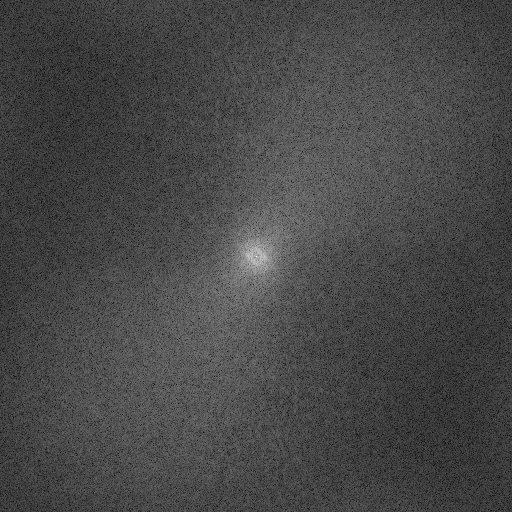
\includegraphics[width=\linewidth]{img/ch6/leopard_generated_frequencies.png}
%     \caption{} \label{fig:1b}
%   \end{subfigure}
%   \begin{subfigure}{0.24\textwidth}
%     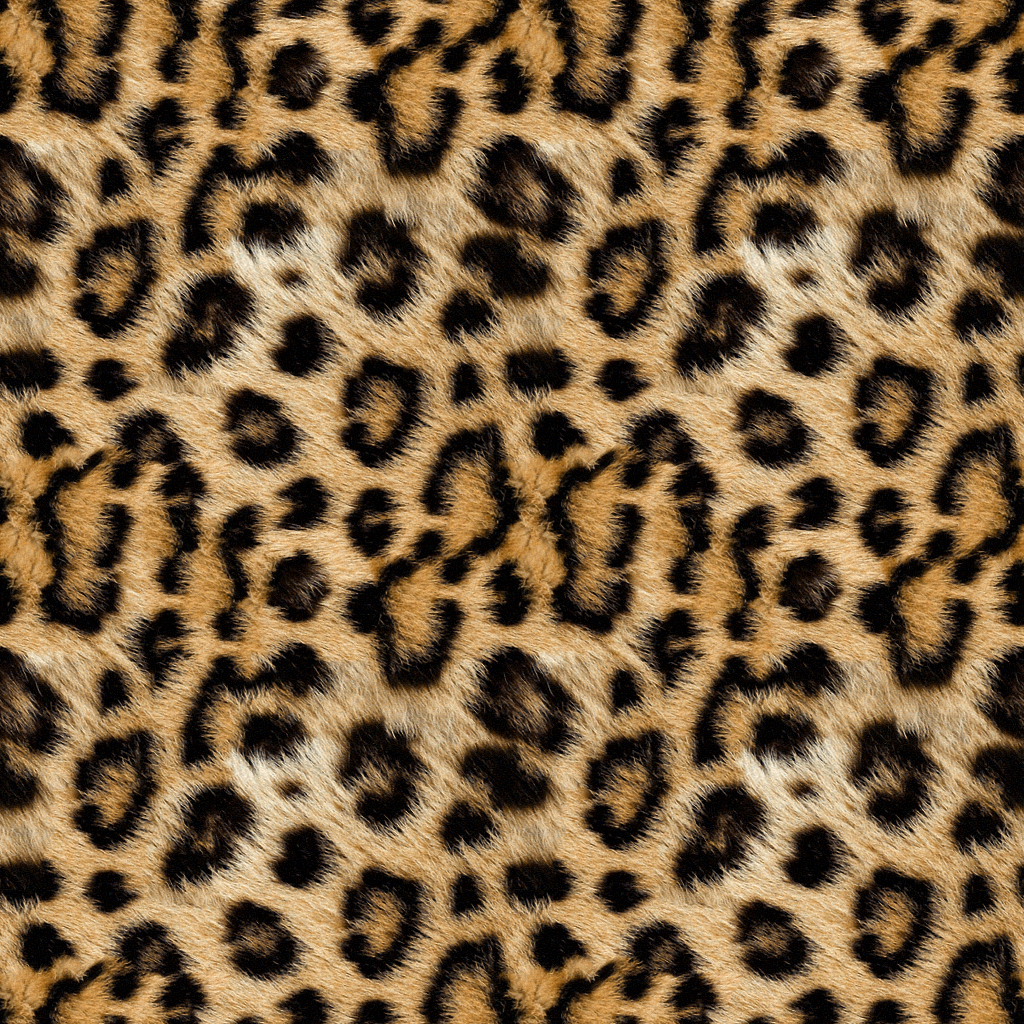
\includegraphics[width=\linewidth]{img/ch6/mnet_extrapolation.png}
%     \caption{} \label{fig:1c}
%   \end{subfigure}
%   \begin{subfigure}{0.24\textwidth}
%     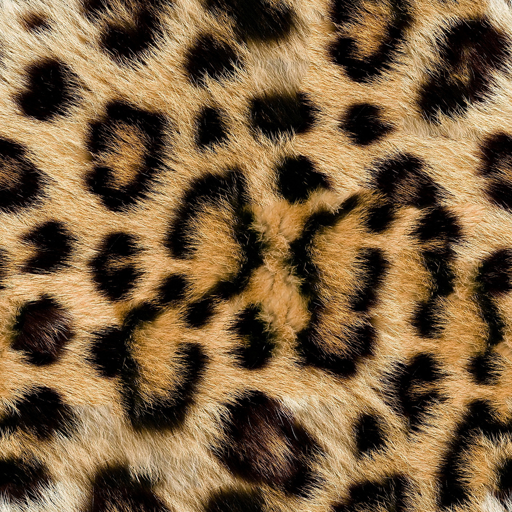
\includegraphics[width=\linewidth]{img/ch6/leopard-train-data.png}
%     \caption{} \label{fig:1d}
%   \end{subfigure}
% \caption{(A) Chosen frequencies for initialization; (B) Fourier transform of the trained model; (C) Seamless reconstruction in $[-2, 2]^2$; (D) Training data in $[-1, 1]^2$.}
% \label{f:tileable_leopard_comparison_siren}
% \end{figure}

% % We now present an initialization scheme for periodic INRs based on a Fourier series interpretation.

% % % The first layer of a sinusoidal INR projects the input coordinates into a list of sines (Eq.~\ref{e-firstlayer}). Next, we show that in a shallow network, this gives the frequencies of the signal represented by a Fourier series. Thus, the initialization of the first layer is important for network performance.
% % Following the conclusions of Theorem~\ref{t-periodic}, we define the first layer's frequencies to be integer multiples of a period.

% % Let $\gt{f}\!:\!\R^2\!\to\! \R$ be a periodic image (the \textit{ground-truth}) with period~$P$ and ${f}\!:\!\R^2\!\to\! \R$ be a periodic INR.
% % To define the integer matrix $k_{jl}$ of the first layer of $f$ we follow ideas from Fourier~series.
% % % . Fourier series 
% % If $\gt{f}\in L^1(P)$, the \textit{Fourier theorem} says that it expands in a series:
% % \begin{align}\label{e-fourier-expansion}
% %     \gt{f}(x)=\sum_{\textbf{k}\in \Z^2} c_\textbf{k} \text{e}^{i\dot{\omega_{{\textbf{k}}}}{ x}},
% % \end{align}
% % where $c_\textbf{k}$ are the \textit{Fourier coefficients}, and $\omega_{\textbf{k}}=2\pi\left(\frac{k_1}{P_1}, \frac{k_2}{P_2}\right)$ with $\textbf{k}=(k_1,k_2)$. 
% % %
% % In practice, we truncate the Fourier series summing over the integers $\textbf{k}\in[-B, B]^2$, where $B$ is a \textit{bandlimit}.
% % %

% % On the other hand, assuming $f$ to be a network with a single layer (Eq~\eqref{e-fourier_series}) and adding $\frac{\pi}{2}$ to the biases, we obtain:
% % \begin{align}\small
% %     f(x) &=  \frac{a_0}{2} + \sum_{k=1}^{n} a_k  \cos\big(\dot{\omega_k}{ x}+ \varphi_k\big)\\
% %     &=  c_0 + \sum_{k=1}^{n} c_k  \text{e}^{i\dot{\omega_{{k}}}{ x}}+ \sum_{k=-n}^{-1} c_k  \text{e}^{i\dot{-\omega_{\abs{k}}}{ x}},\label{e-mlp2complex}
% % \end{align}
% % where $c_k=\frac{a_{\abs{k}}}{2}\text{e}^{\text{sign}(k)i\varphi_{\abs{k}}}$ with $\varphi_0=0$, and $\omega_{j}=2\pi\left(\frac{k_{j,1}}{P_1}, \frac{k_{j,2}}{P_2}\right)$. 
% % %
% % % . Frequency initialization
% % Thus, for $f$ to approximate the truncated series in Eq.~\eqref{e-fourier-expansion}, we can set
% % the integers $k_{j}$ in a set $\textbf{K}\subset [-B,B]^n$ such that $-\textbf{K} = [-B,B]^n\setminus \textbf{K}$.

% % % % . Other parameters...
% % When $f$ contains hidden layers, we initialize its parameters following the scheme in ~\cite{sitzmann2019siren}. 
% % Notice that we initialized $f$ with a finite number of frequencies in the frequency set $\textbf{K}$. However, 
% % the layer composition produces many other frequencies as the depth of the network increases.
% % Equation~\ref{e-expansion} justifies this claim.

% Using our method, we observe that a single sample from the equivalence class defined by the periodicity suffices to reconstruct the image without additional regularization. 
% To illustrate this, we construct a mask by randomly selecting a pixel and then excluding all pixels corresponding to it based on the pattern's period. This process repeats until no further pixels can be sampled, resulting in a mask covering $1/4$ of the total pixels. Figure \ref{f:masked_recontruction} presents the training data, where the black pixels were removed from training, and the learned texture in $[2, 6]^2$. In this case, the training still considers the interval $[-1, 1]$ but the period $P$ is set to $1$. Even under these conditions, our method captures the underlying periodicity.

% % \begin{figure}[h]{\textwidth}
% %     \centering
% %     \includegraphics[width=0.40\linewidth]{img/victorian/stochastic_mask.png}
% %     \includegraphics[width=0.40\linewidth]{img/victorian/extrapolation_randommask.png}
% %     \caption{The masked input data, where the black pixels were removed from training (left). The network reconstruction (right).~\\
% %     }
    
% % \end{figure}


% \begin{figure}[h]
%     \centering
%     \begin{subfigure}[b]{0.40\textwidth}
%         \centering
%         \includegraphics[width=\textwidth]{img/ch6/stochastic_mask.png}
%         % \caption{$\omega_0=2$ Hz}
%     \end{subfigure}
%     \begin{subfigure}[b]{0.40\textwidth}
%         \centering
%         \includegraphics[width=\textwidth]{img/ch6/extrapolation_randommask.png}
%         % \caption{$\omega_0=4$ Hz}
%         % \label{fig:16x-zoom-1hl-16hf-2hz}
%     \end{subfigure}
%     \caption{The masked input data, where the black pixels were removed from training (left). The network reconstruction (right).}
%     \label{f:masked_recontruction}
% \end{figure}


\section{Multiresolution Periodic Representation}


This periodic behavior is also observed across levels of details of a multiresolution INR. Regarding the frequency initialization of each multiresolution stage, we split the frequency set $\textbf{K}$ in subsets sorted by length. Thus, we initialize subsequent stages using only frequencies in subsets that were not chosen in previous stages enforcing the early stages to contain the lower frequencies, then as stages advance we add the higher frequencies.
% when using a multistage network such as MR-Net \cite{paz2022, paz2023mr}. 
Figure \ref{f:mr-periodic} showcases 5 levels of detail of an M-Net model trained with 6 stages in $[-1, 1]^2$ and sampled in $[-2, 2]^2$. The input image has a resolution of $1024^2$ pixels and $8$ bits per color channel in RGB space. The results were produced by training a $6$ stage M-Net architecture \cite{paz2022} using a Gaussian pyramid representation of the data. We explored network stages with a single hidden layer, and heterogeneous width, as experiments have indicated that we need fewer parameters to fit an image of lower resolution and low frequency details. The initialization follows the method described in the section 4. Table \ref{tab:mnet-architecture} details the the band limits of the first layer, the architecture of the hidden layer (number of values received and number of values produced), and the maximum number of epochs that each stage was trained. We used the Adam optimizer with a learning rate of $10^{-3}$.

\begin{figure}[!ht]
    \centering
    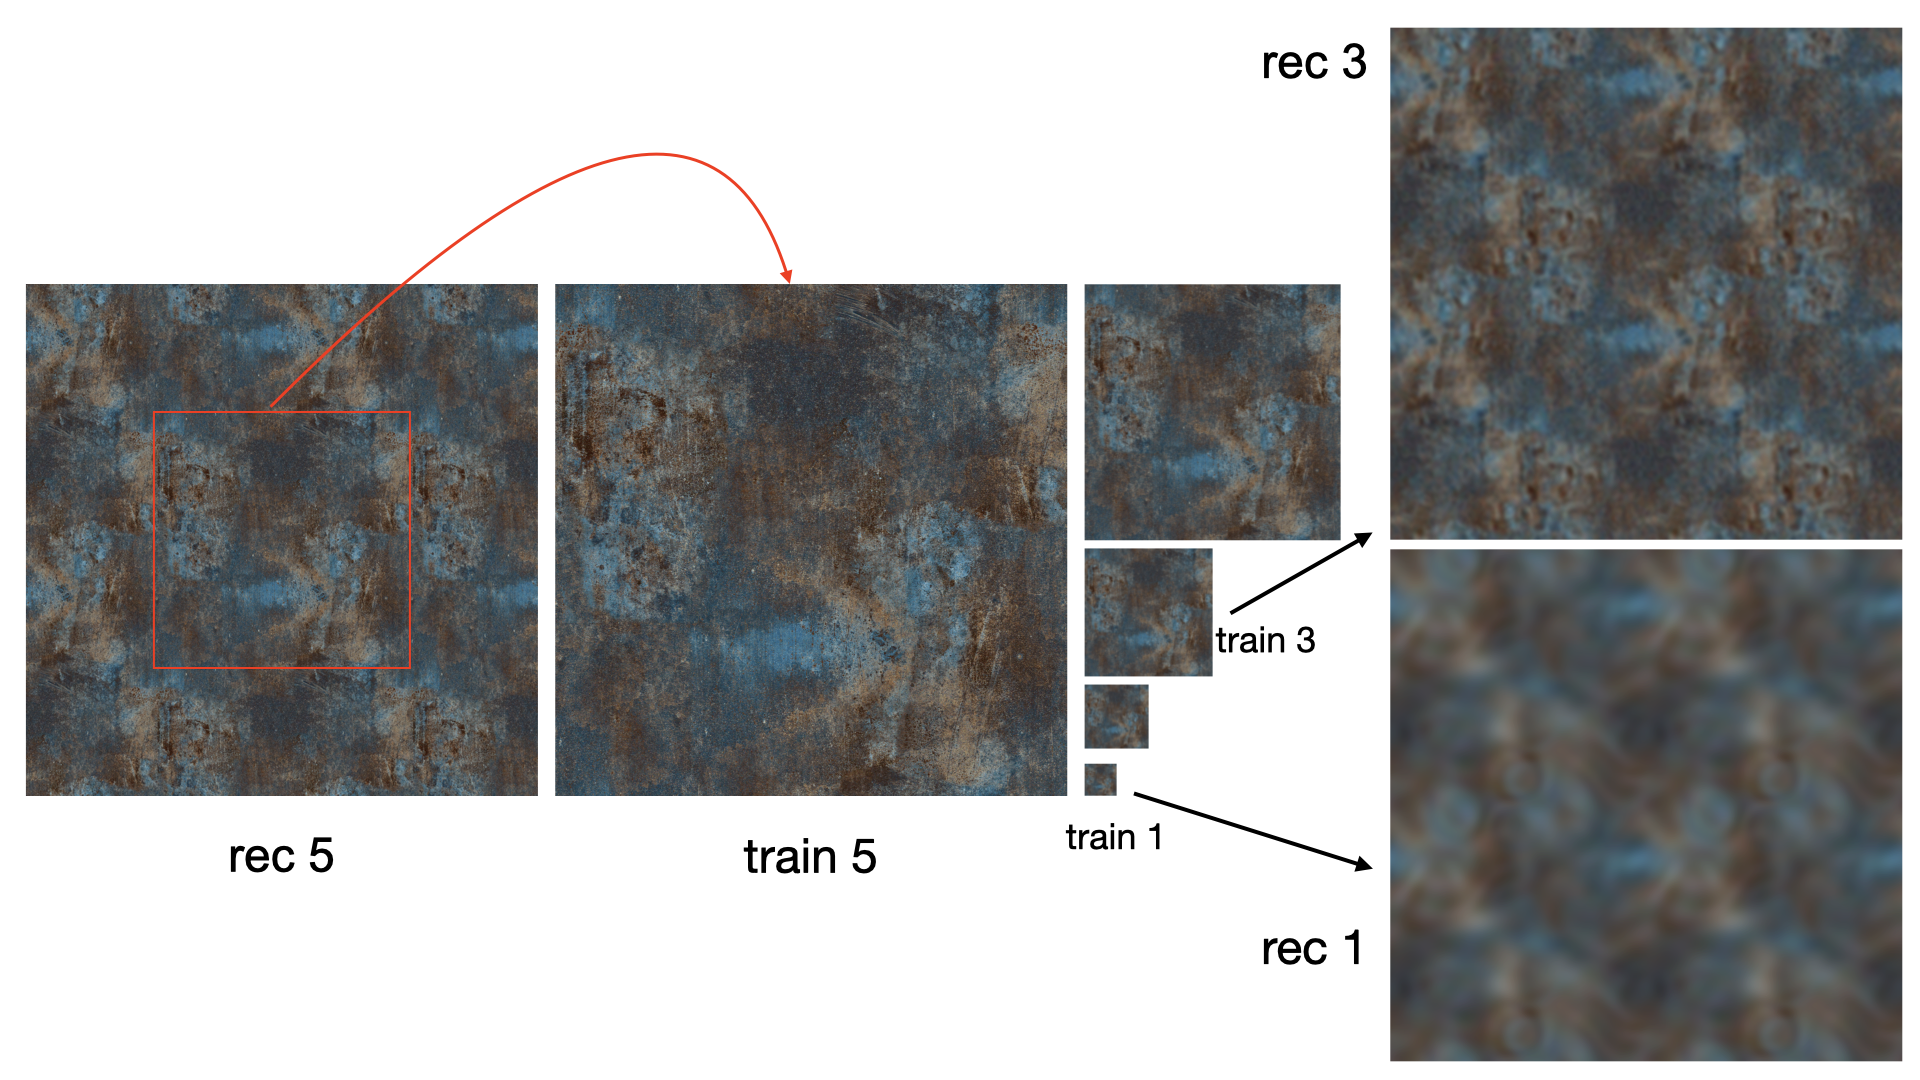
\includegraphics[width=0.90\linewidth]{img/ch6/diagram.png}
    \caption{In the center, the training data for stages 1 (train 1) to 5 (train 5). On the left, the extrapolated reconstruction of the 5th level of detail highlights how the training data (train 5) aligns with the center of the reconstruction (rec 5). On the right, reconstructions of the 1st and 3rd levels of detail, are generated by sampling the networks at a higher resolution grid.}
    \label{f:mr-periodic}
\end{figure}


\begin{table}[h]
\small
\begin{tabular}{|l|c|c|c|c|}
\hline
\textbf{Stage} & \multicolumn{1}{l|}{\textbf{Band-Limit}} & \multicolumn{1}{l|}{\textbf{Hidden Input}} & \multicolumn{1}{l|}{\textbf{Hidden Output}} & \multicolumn{1}{l|}{\textbf{Epochs}} \\ \hline
 0     & $[0, 3]\times[-3, 3]$                       & 24                                & 32          &  1600                     \\
 1     & $[0, 6]\times[-6, 6]$                       & 48                                & 32         &  1200                      \\
 2     & $[0, 12]\times[-12, 12]$                     & 80                                & 64             & 1000                   \\
 3     & $[0, 24]\times[-24, 24]$                     & 192                               & 160           &   800                  \\
 4     & $[0, 56]\times[-56, 56]$                     & 384                               & 256             &  600                 \\
 5     & $[0, 128]\times[-128, 128]$                   & 1024                              & 512            &   400                 \\ \hline
\end{tabular}
\caption{Hyperparameters for training a 6-stages M-Net}
\end{table}\label{tab:mnet-architecture}


Figure \ref{f:rec_gt} presents a qualitative comparison between the original image and the reconstructed image at the finest level using our method. On visual inspection, the images exhibit a high degree of similarity, closely resembling each other at the original resolution. To provide a quantitative assessment, we computed the Peak Signal-to-Noise Ratio (PSNR), which yielded a value of 31.8 dB for this specific example. Note that our model achieves this level of fidelity using 855,572 parameters, which is fewer than the total number of pixels in the image, which amounts to 1,048,576. Additionally, the model demonstrates the ability to encode information at multiple scales.

\begin{figure}[h]
\centering
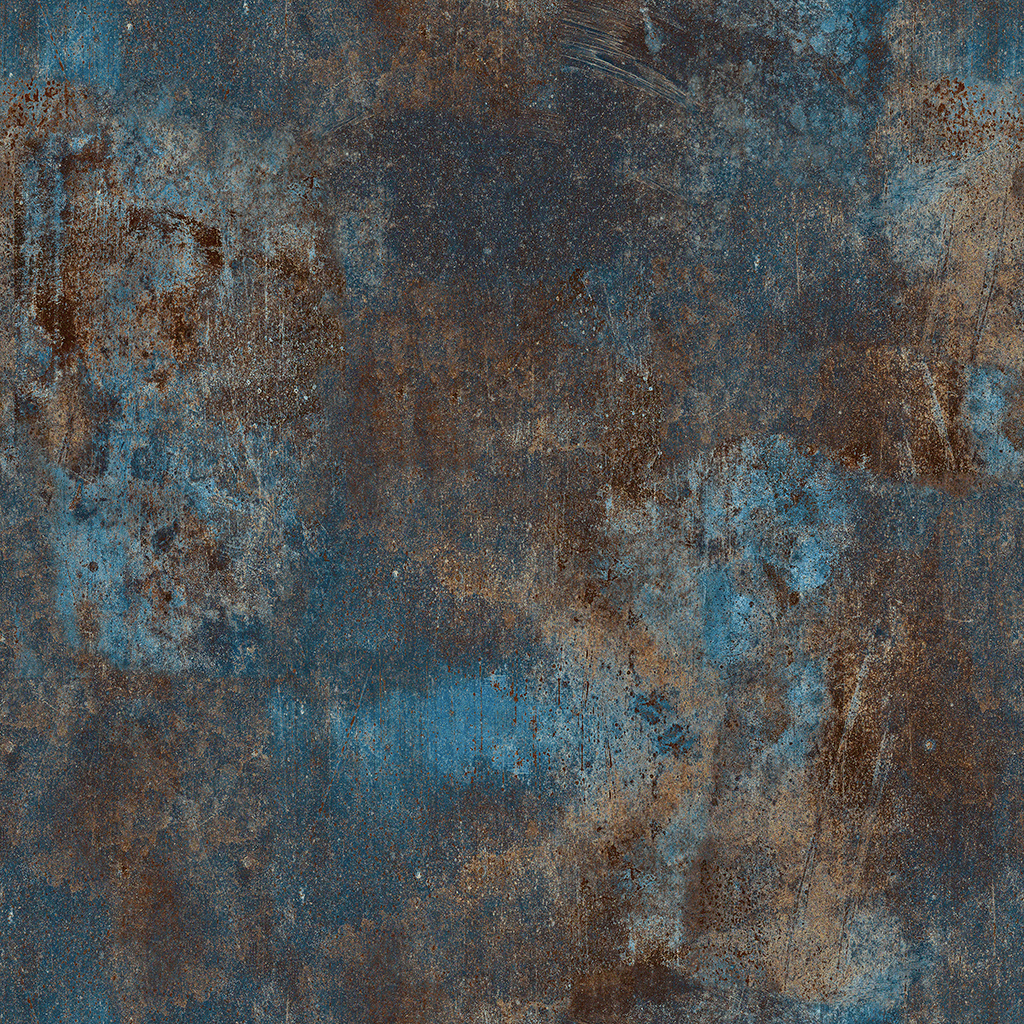
\includegraphics[width=0.42\linewidth]{img/ch6/dirty/gt6.png}
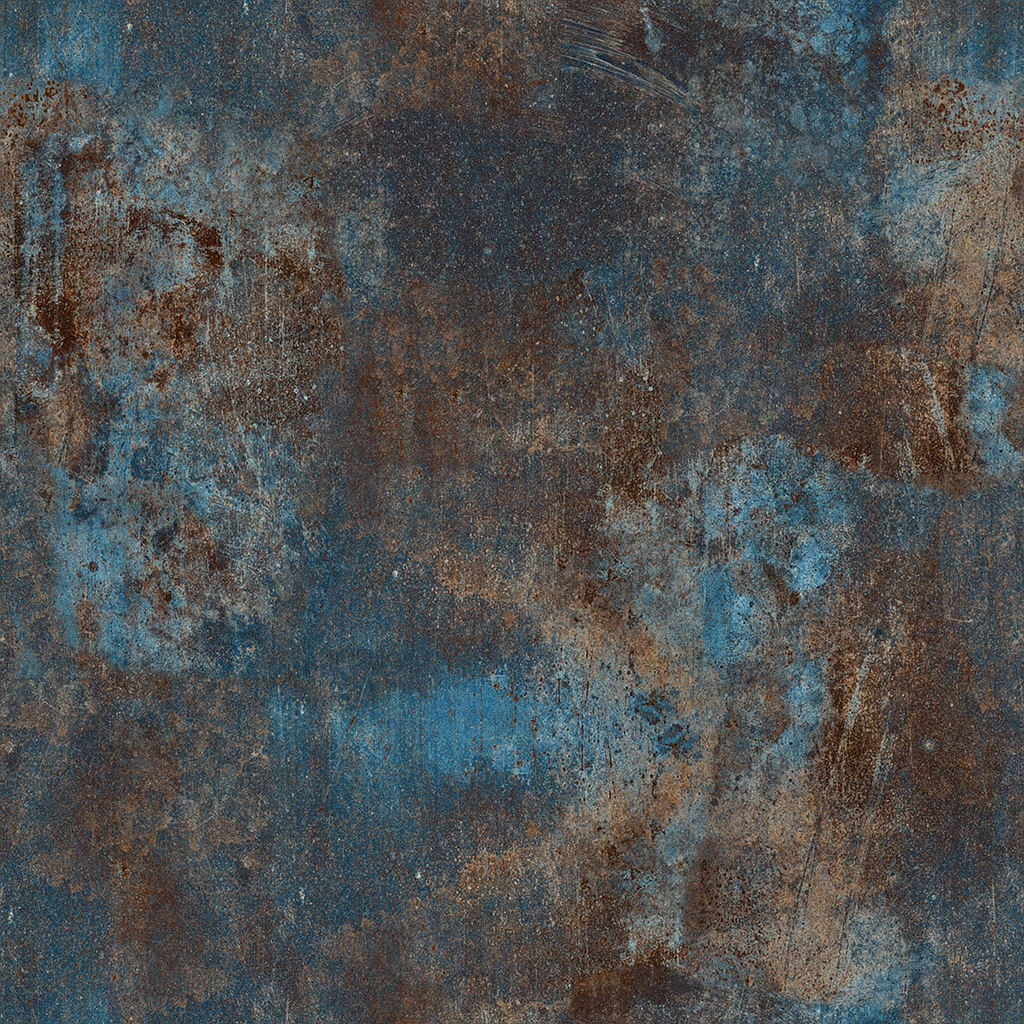
\includegraphics[width=0.42\linewidth]{img/ch6/dirty/detail6.png}
% \centerline{(a) Ours\hfil\hfil(b) Ground Truth}
\caption{Original image (left); reconstruction of the network (right).}
\label{f:rec_gt}
\end{figure}

Figure \ref{f:dirty-extra} shows the 6 levels of detail reconstructed and additional visualizations of the same trained network. Figure \ref{f:copper-extra} shows an additional result of a different image.


\begin{figure}[!h]
\centering

\includegraphics[width=0.16\textwidth]{img/ch6/dirty/train1.png}
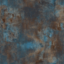
\includegraphics[width=0.16\textwidth]{img/ch6/dirty/train2.png}
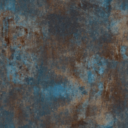
\includegraphics[width=0.16\textwidth]{img/ch6/dirty/train3.png}
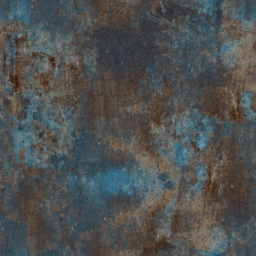
\includegraphics[width=0.16\textwidth]{img/ch6/dirty/train4.png}
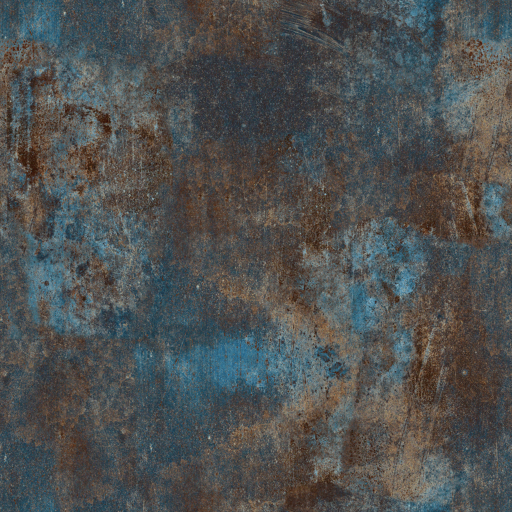
\includegraphics[width=0.16\textwidth]{img/ch6/dirty/train5.png}
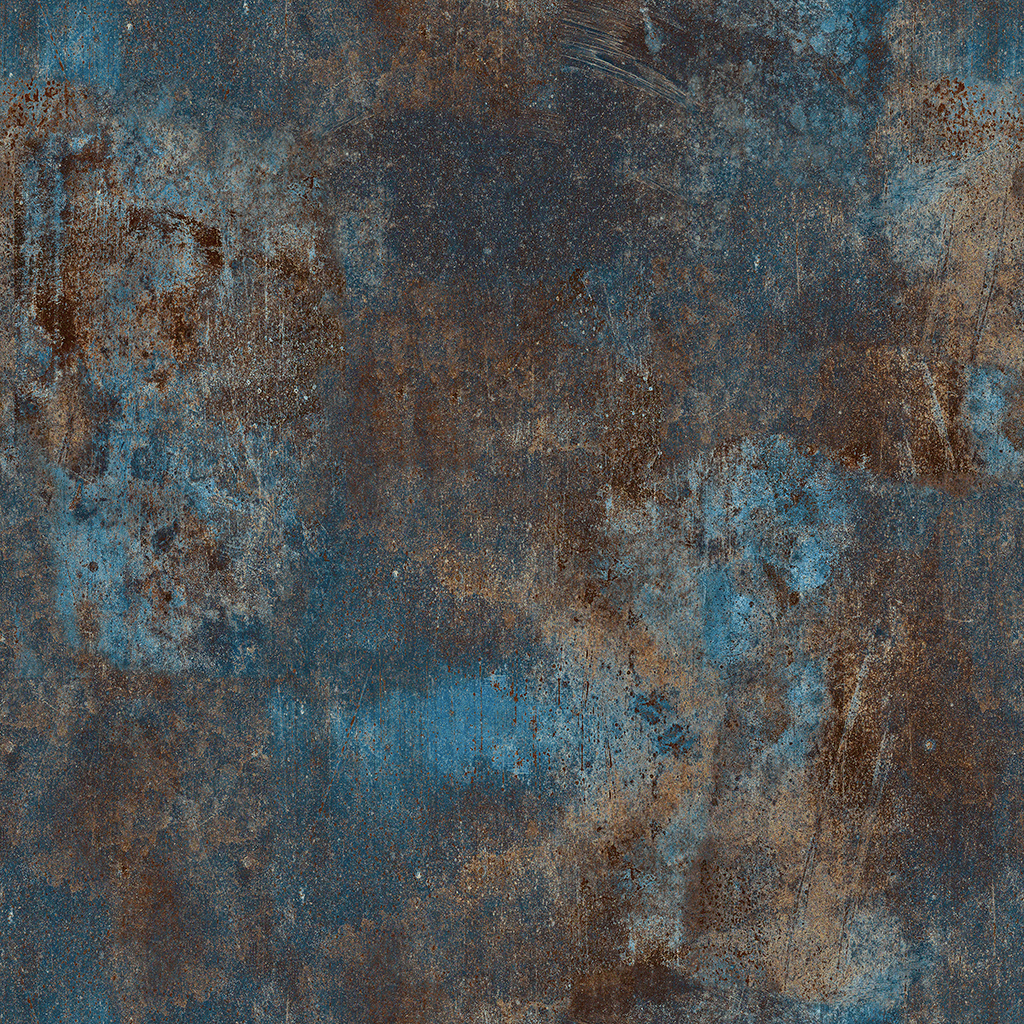
\includegraphics[width=0.16\textwidth]{img/ch6/dirty/train6.png}

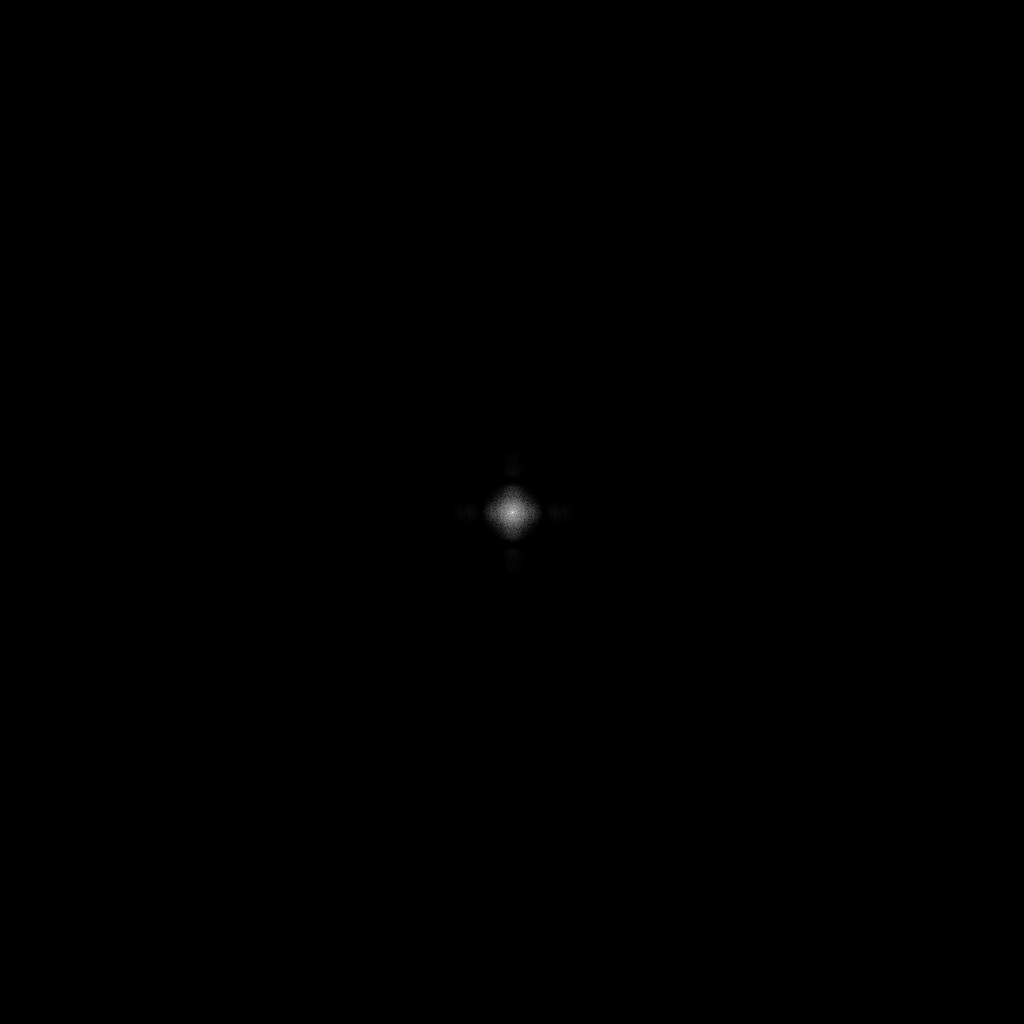
\includegraphics[width=0.16\textwidth]{img/ch6/dirty/gfft1.png}
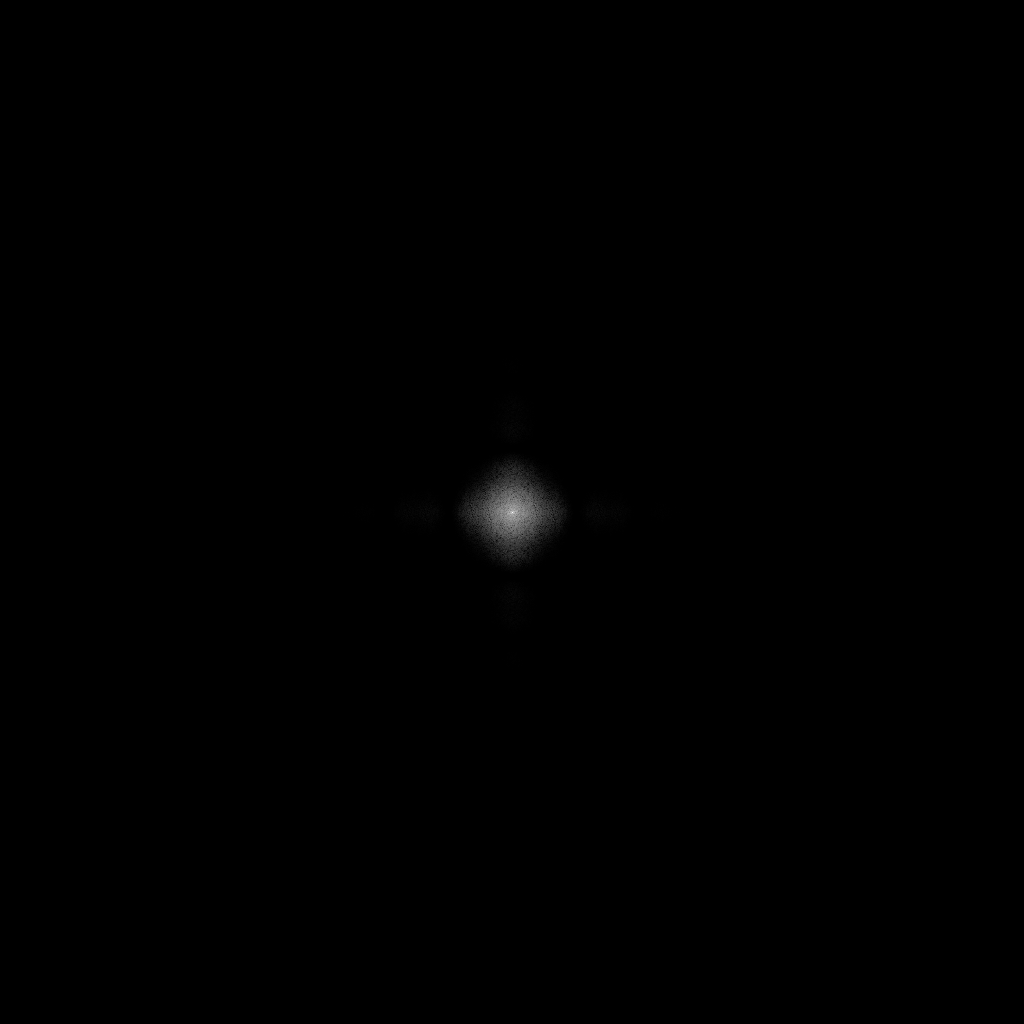
\includegraphics[width=0.16\textwidth]{img/ch6/dirty/gfft2.png}
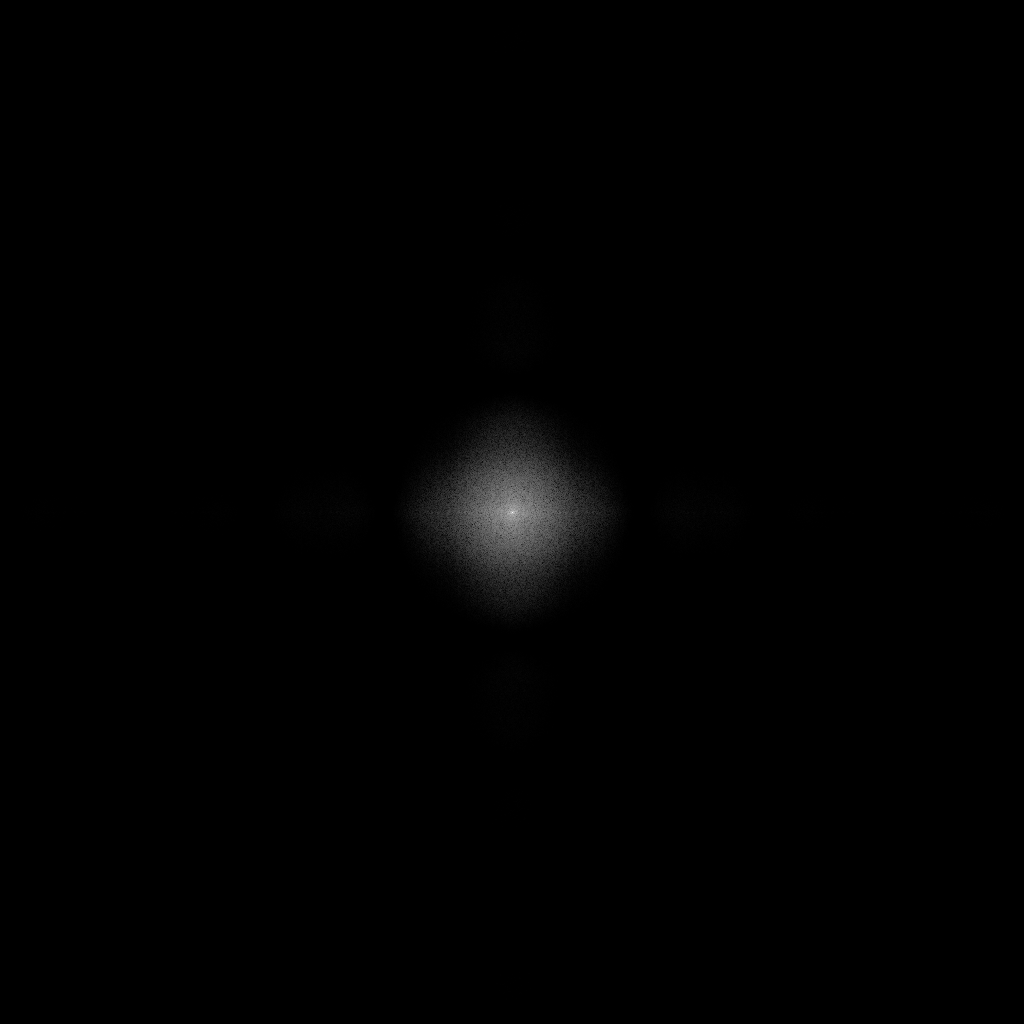
\includegraphics[width=0.16\textwidth]{img/ch6/dirty/gfft3.png}
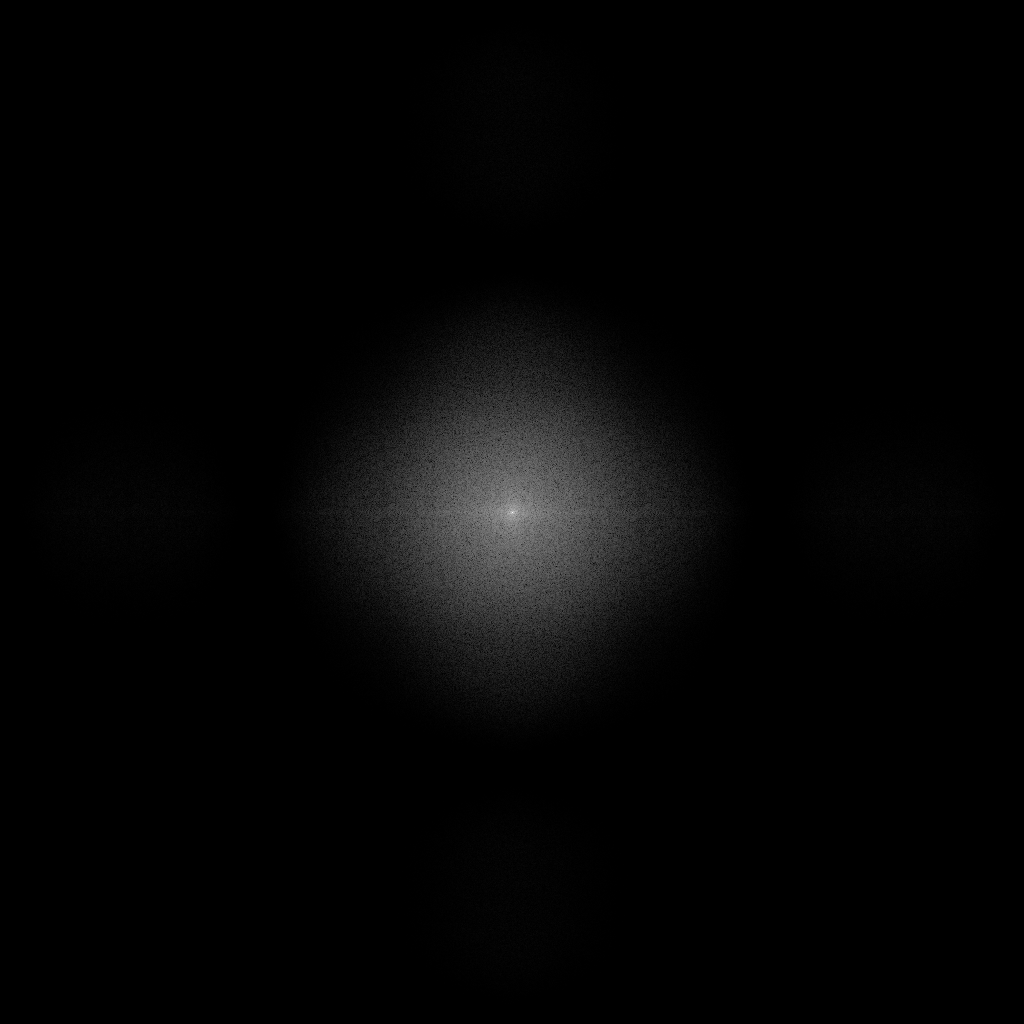
\includegraphics[width=0.16\textwidth]{img/ch6/dirty/gfft4.png}
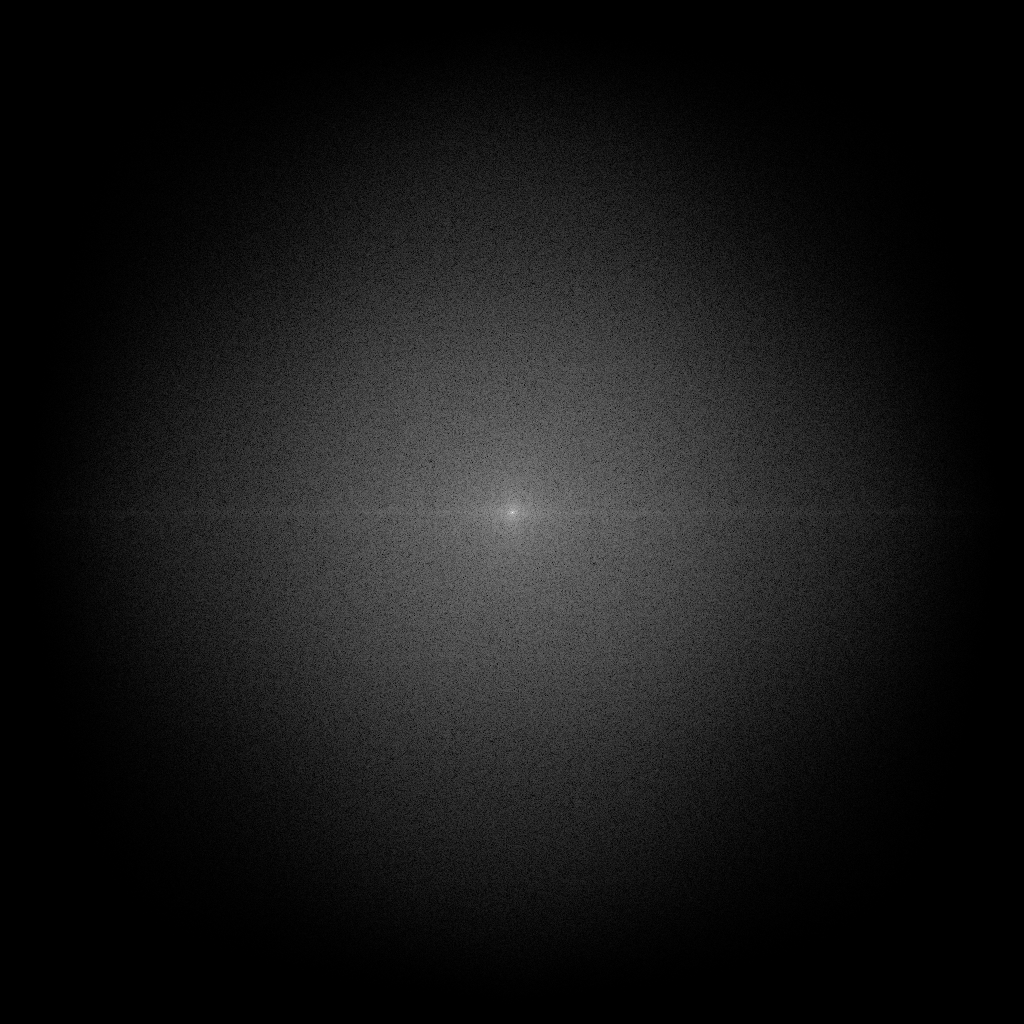
\includegraphics[width=0.16\textwidth]{img/ch6/dirty/gfft5.png}
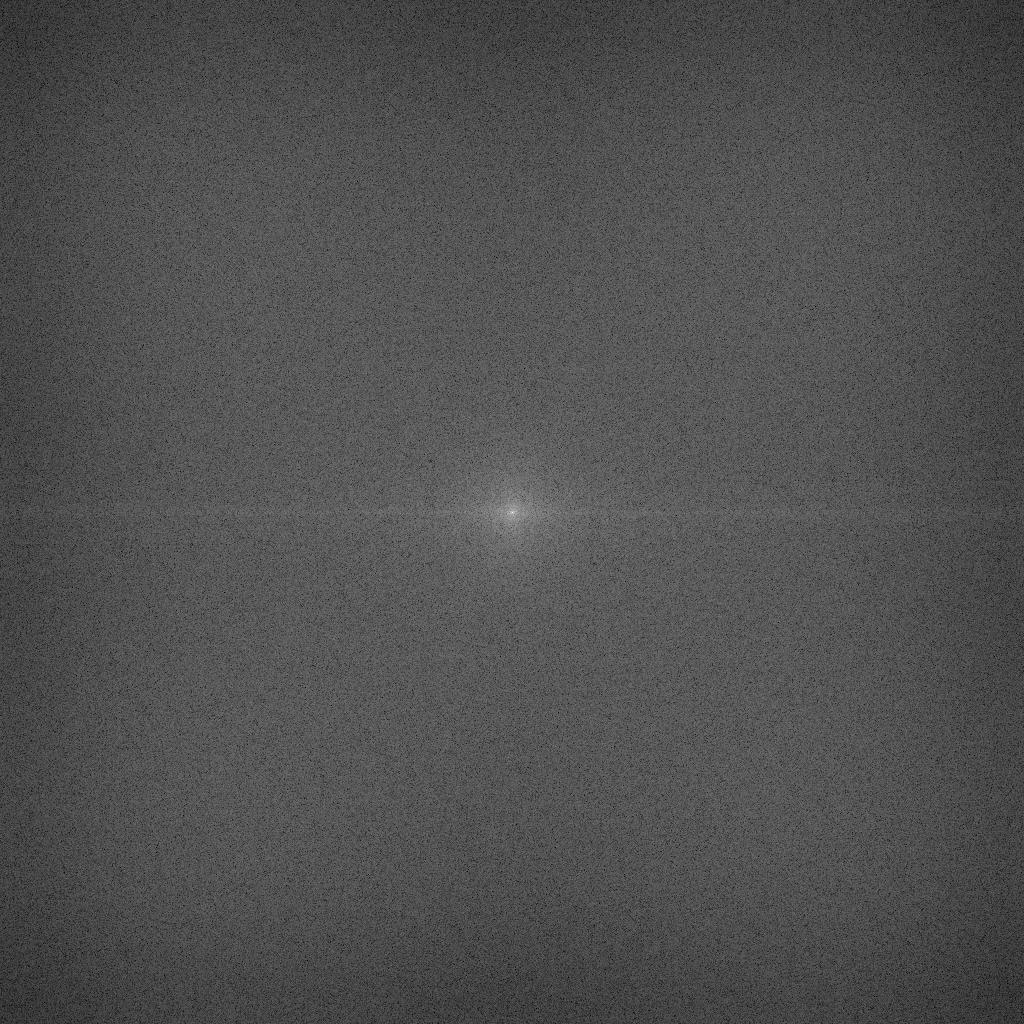
\includegraphics[width=0.16\textwidth]{img/ch6/dirty/gfft6.png}


\includegraphics[width=0.16\textwidth]{img/ch6/dirty/detail1.png}

\includegraphics[width=0.16\textwidth]{img/ch6/dirty/detail2.png}
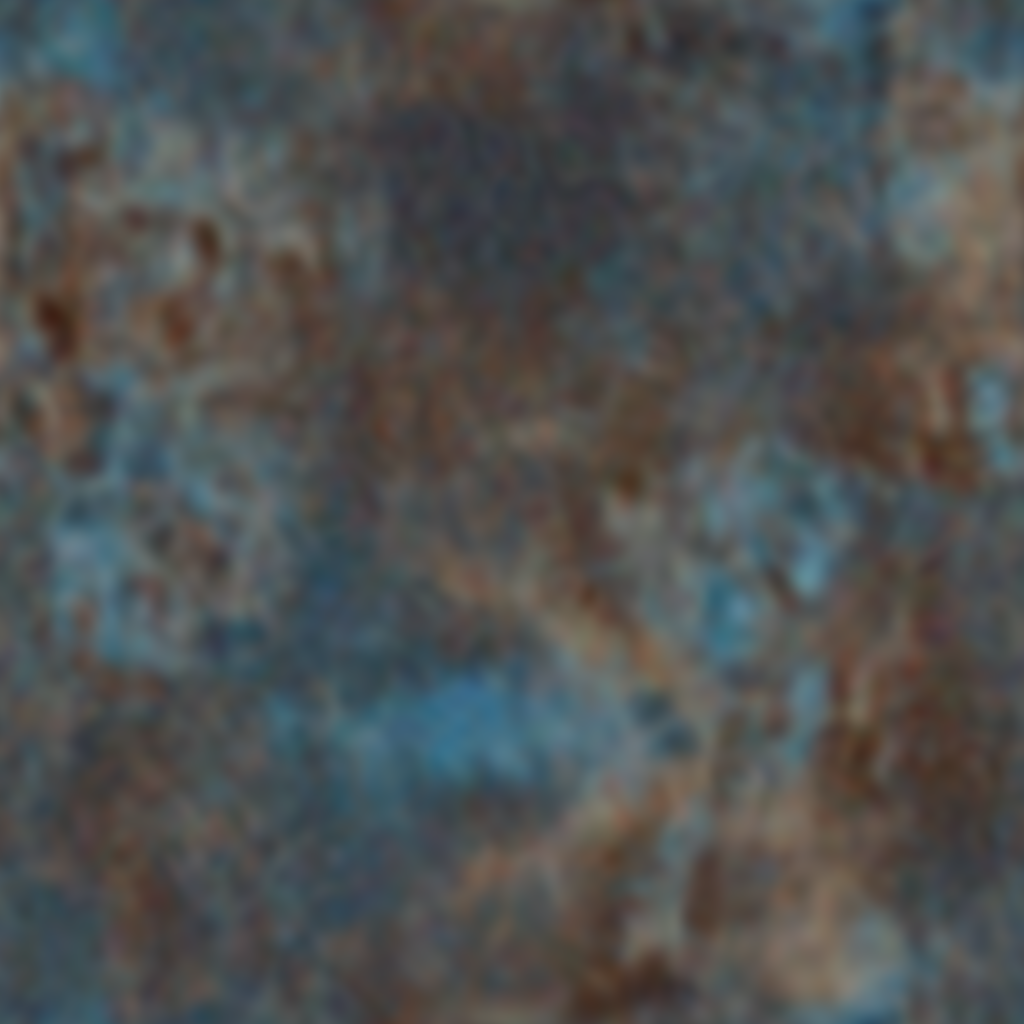
\includegraphics[width=0.16\textwidth]{img/ch6/dirty/detail3.png}
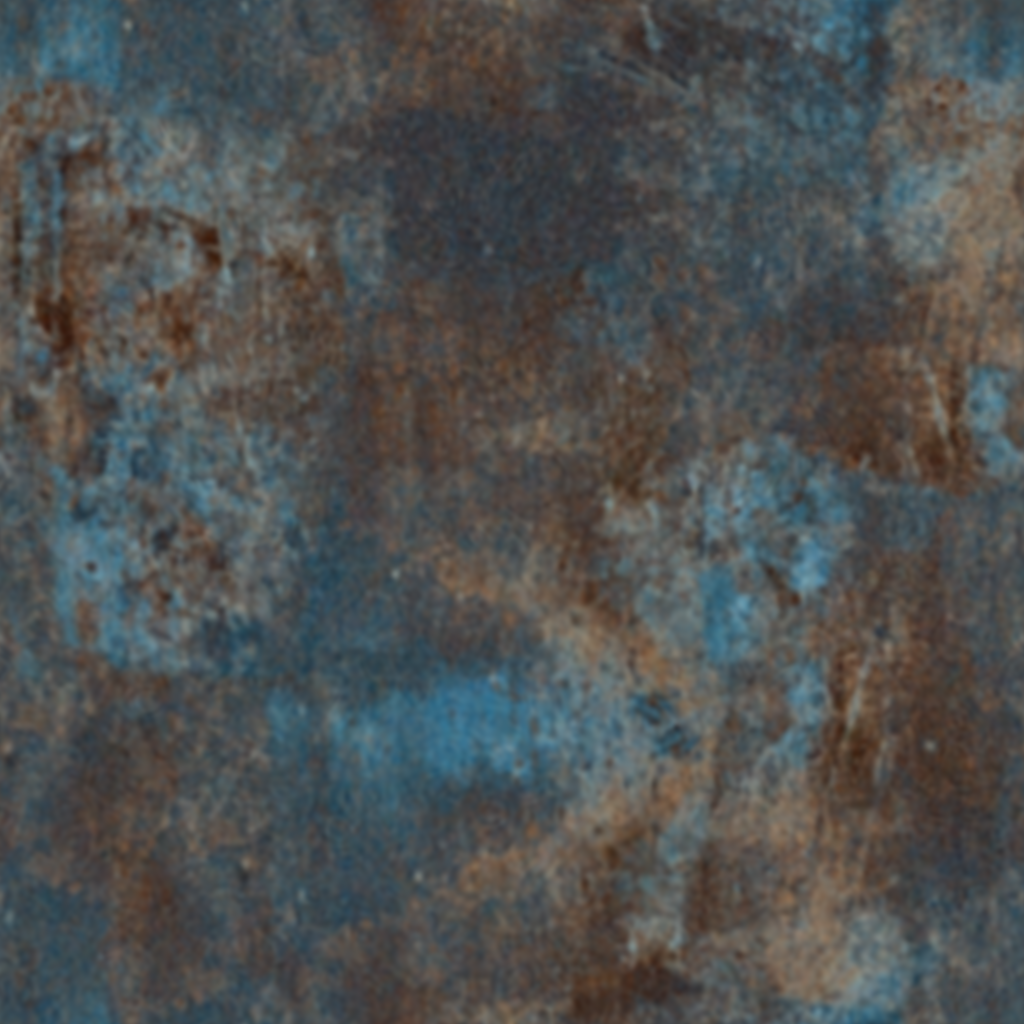
\includegraphics[width=0.16\textwidth]{img/ch6/dirty/detail4.png}
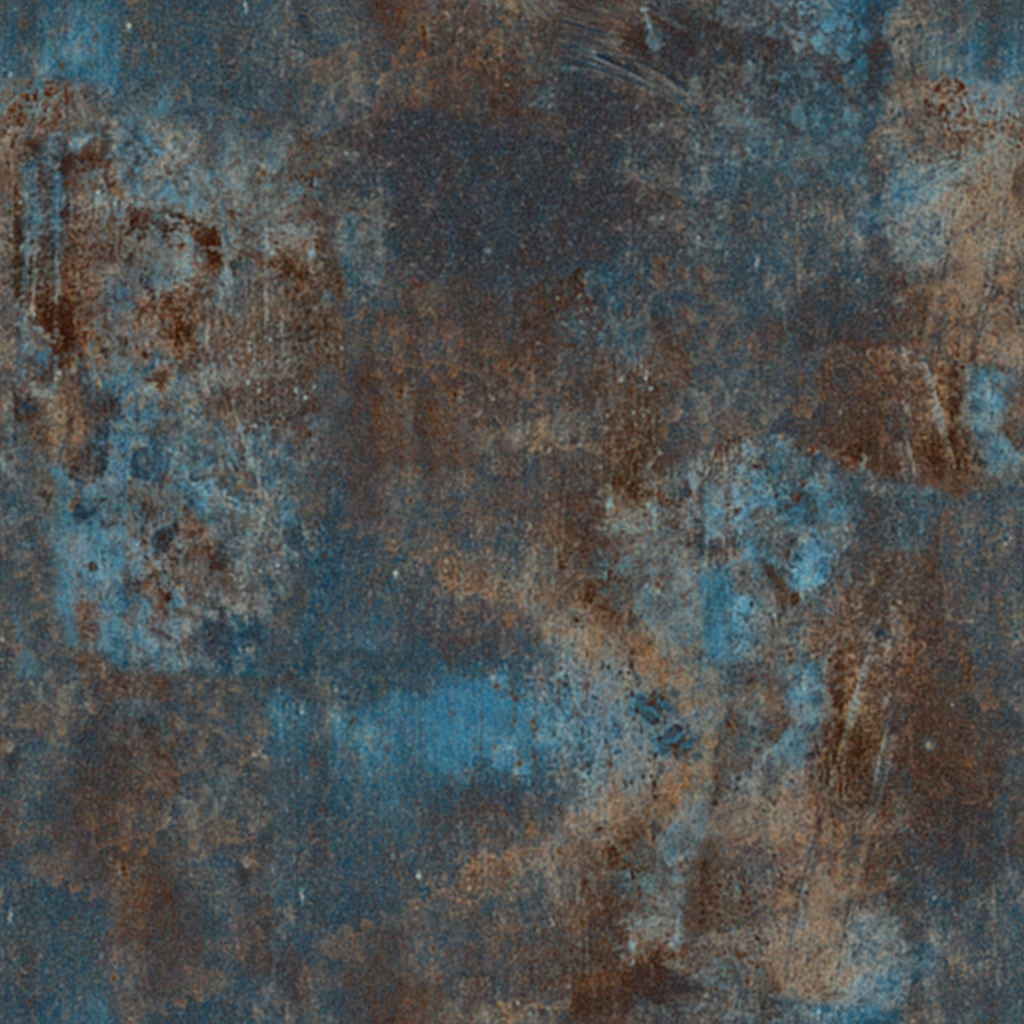
\includegraphics[width=0.16\textwidth]{img/ch6/dirty/detail5.png}
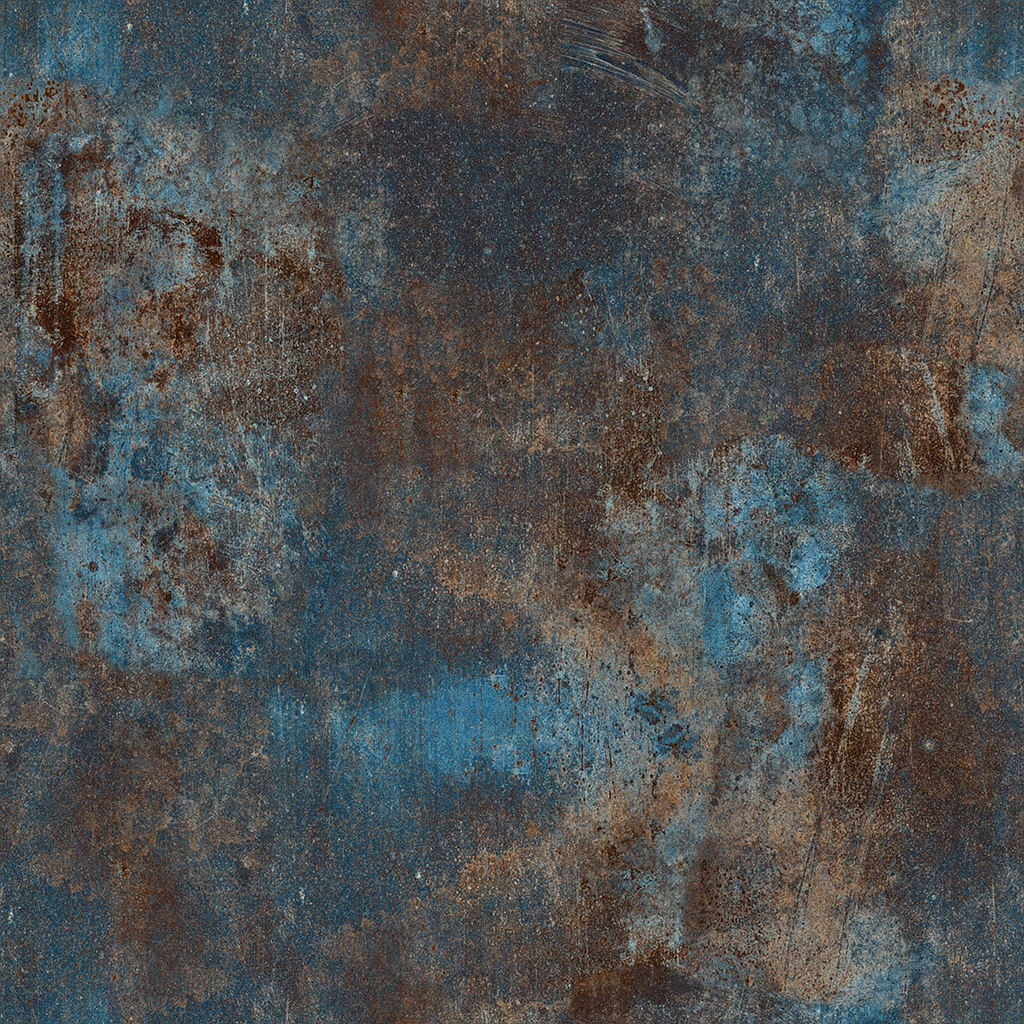
\includegraphics[width=0.16\textwidth]{img/ch6/dirty/detail6.png}

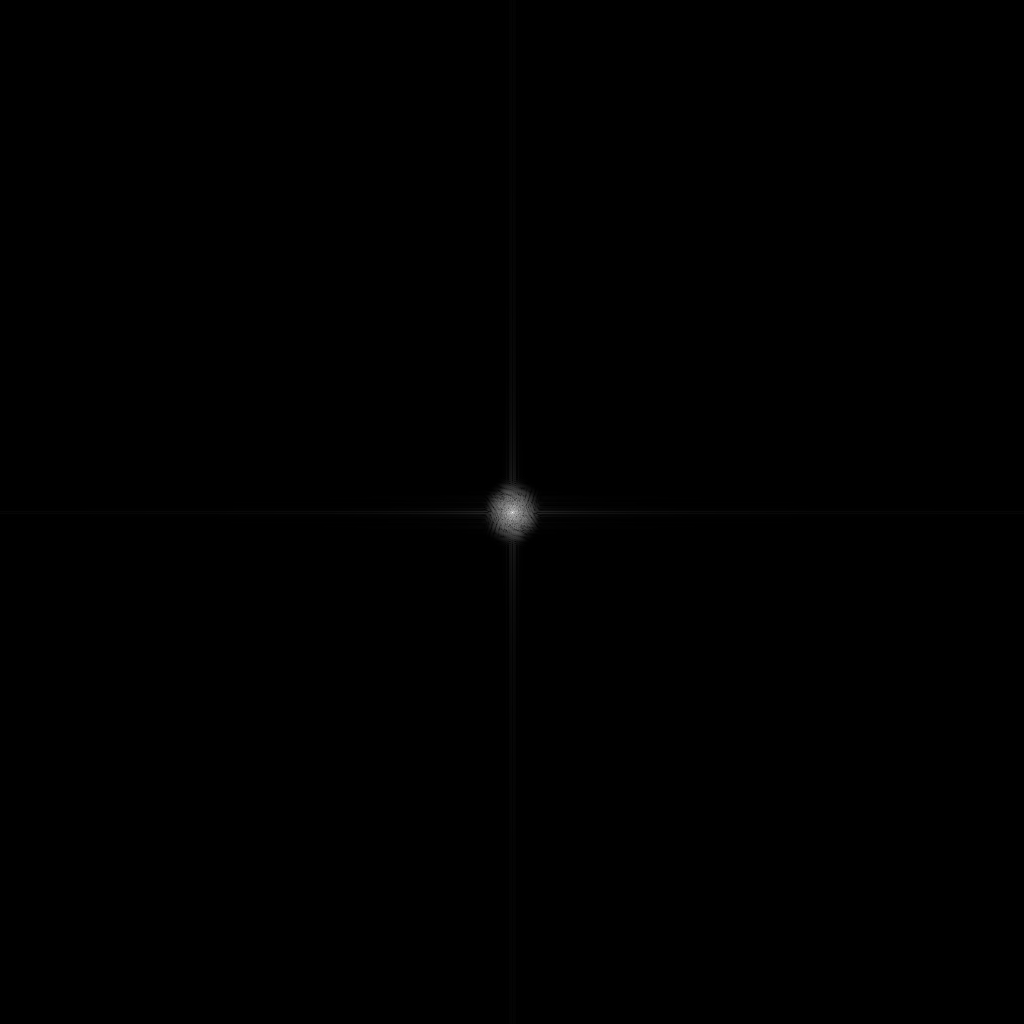
\includegraphics[width=0.16\textwidth]{img/ch6/dirty/fft1.png}
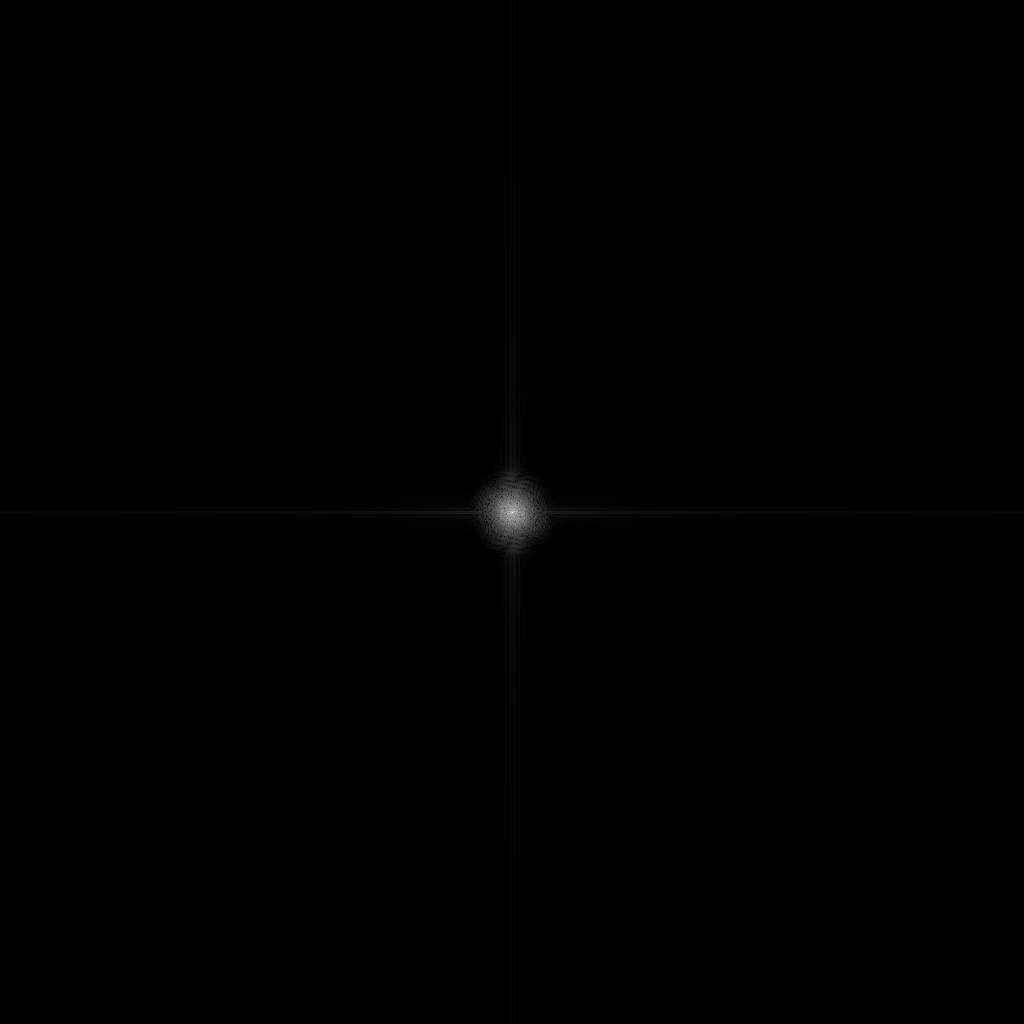
\includegraphics[width=0.16\textwidth]{img/ch6/dirty/fft2.png}
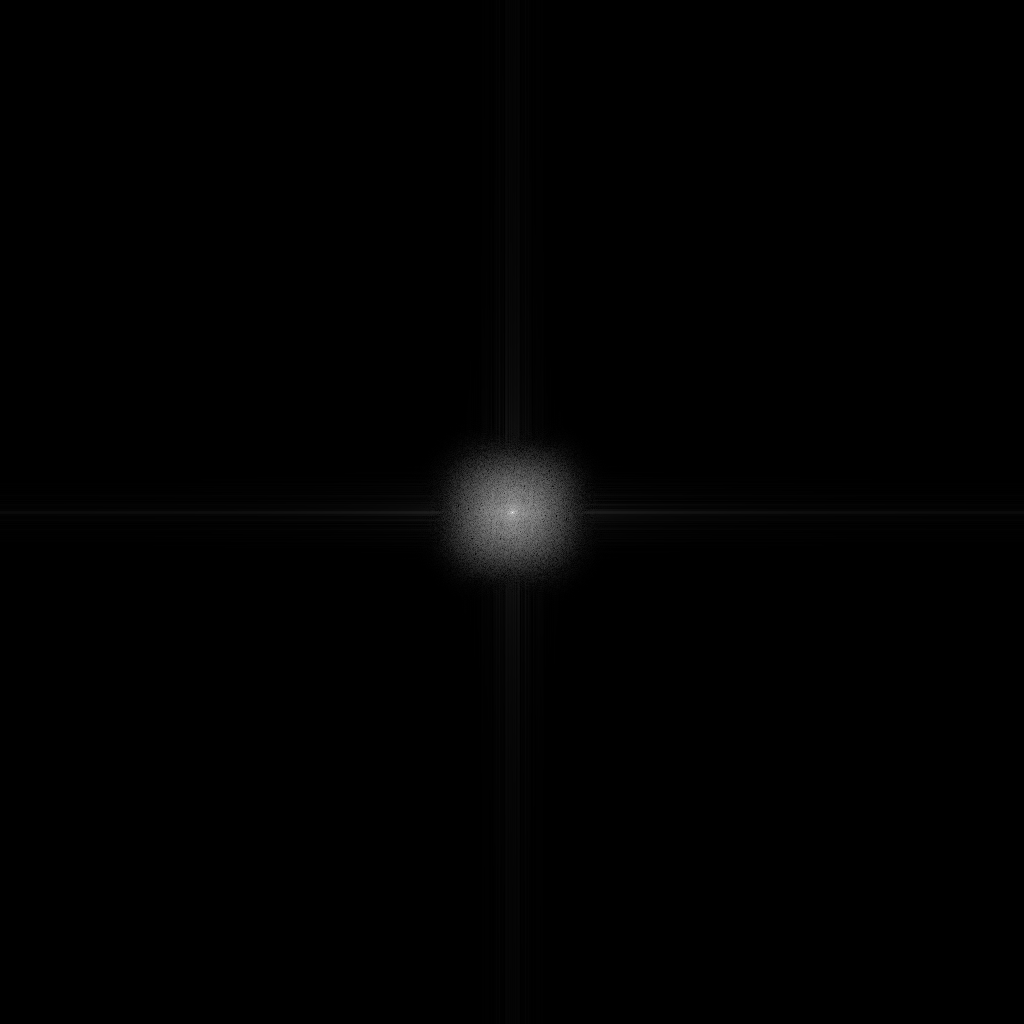
\includegraphics[width=0.16\textwidth]{img/ch6/dirty/fft3.png}
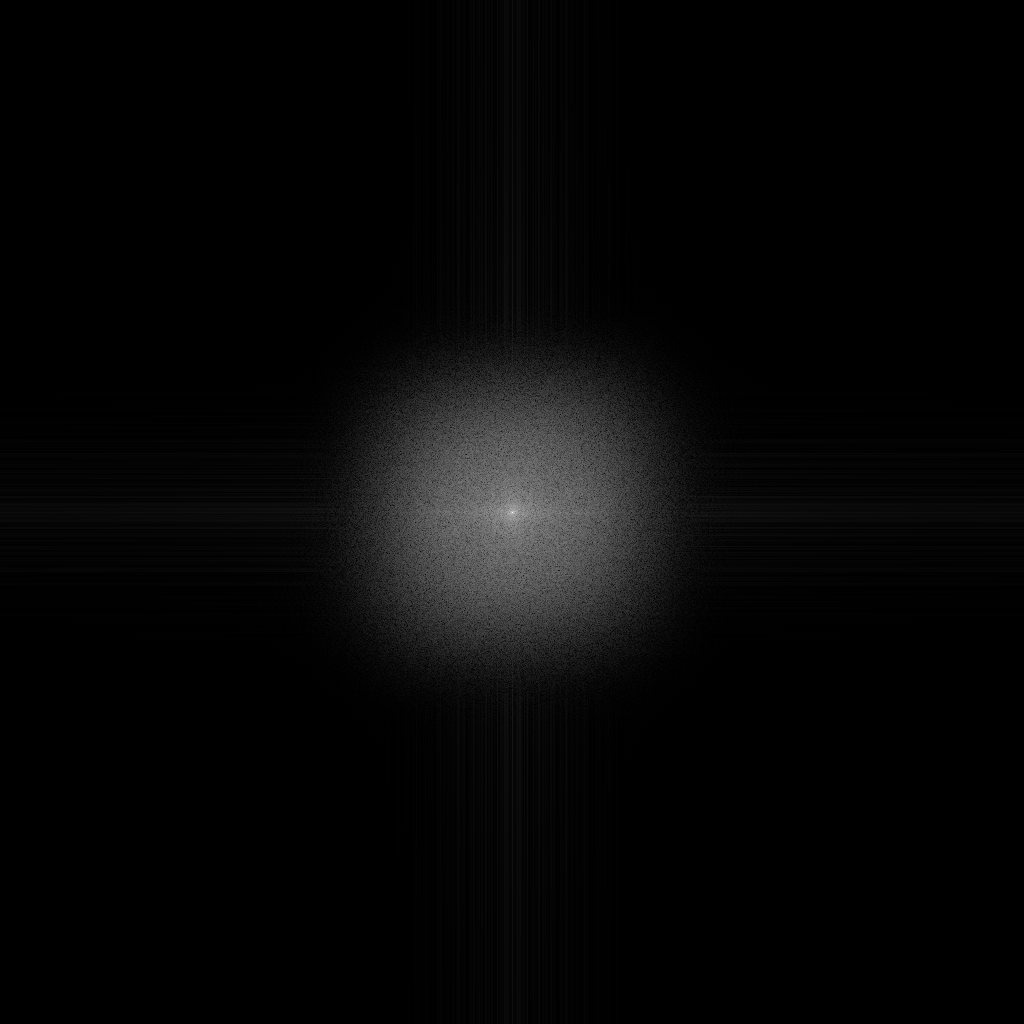
\includegraphics[width=0.16\textwidth]{img/ch6/dirty/fft4.png}
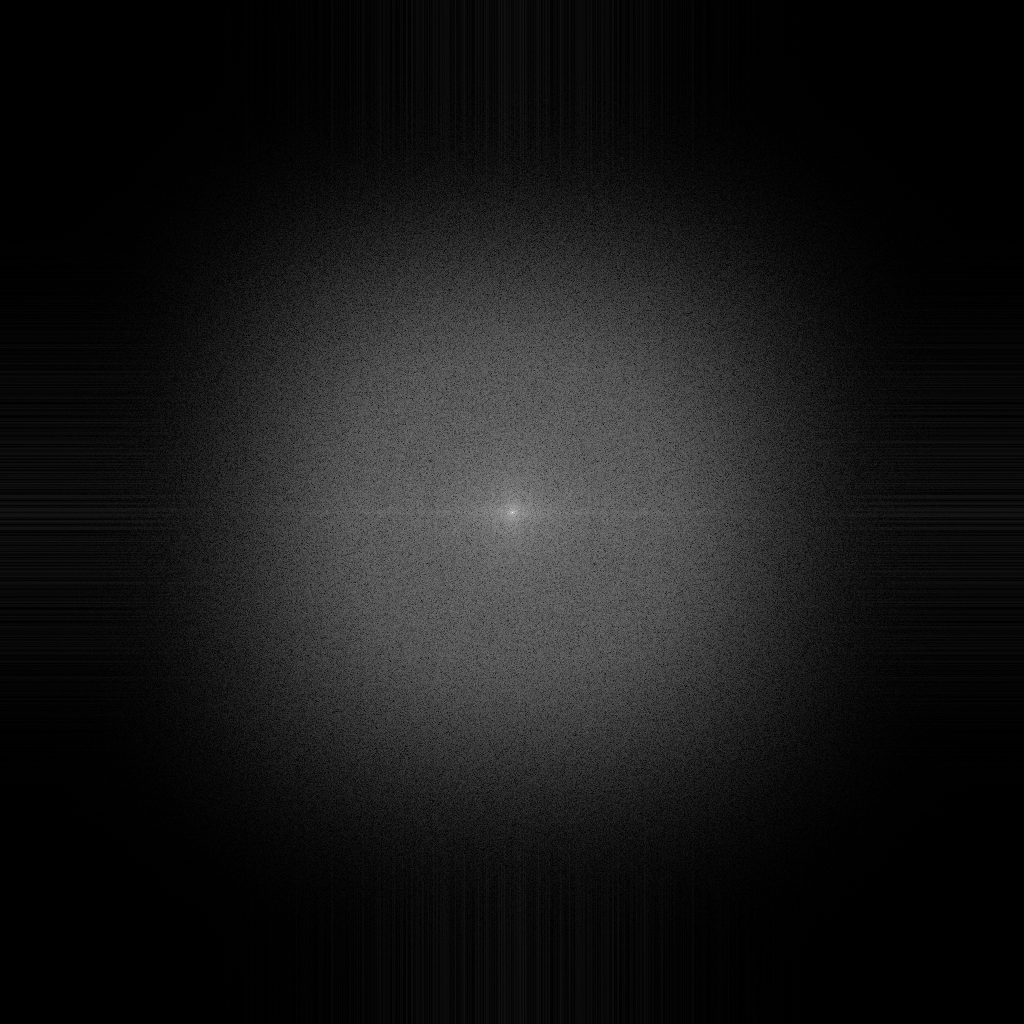
\includegraphics[width=0.16\textwidth]{img/ch6/dirty/fft5.png}
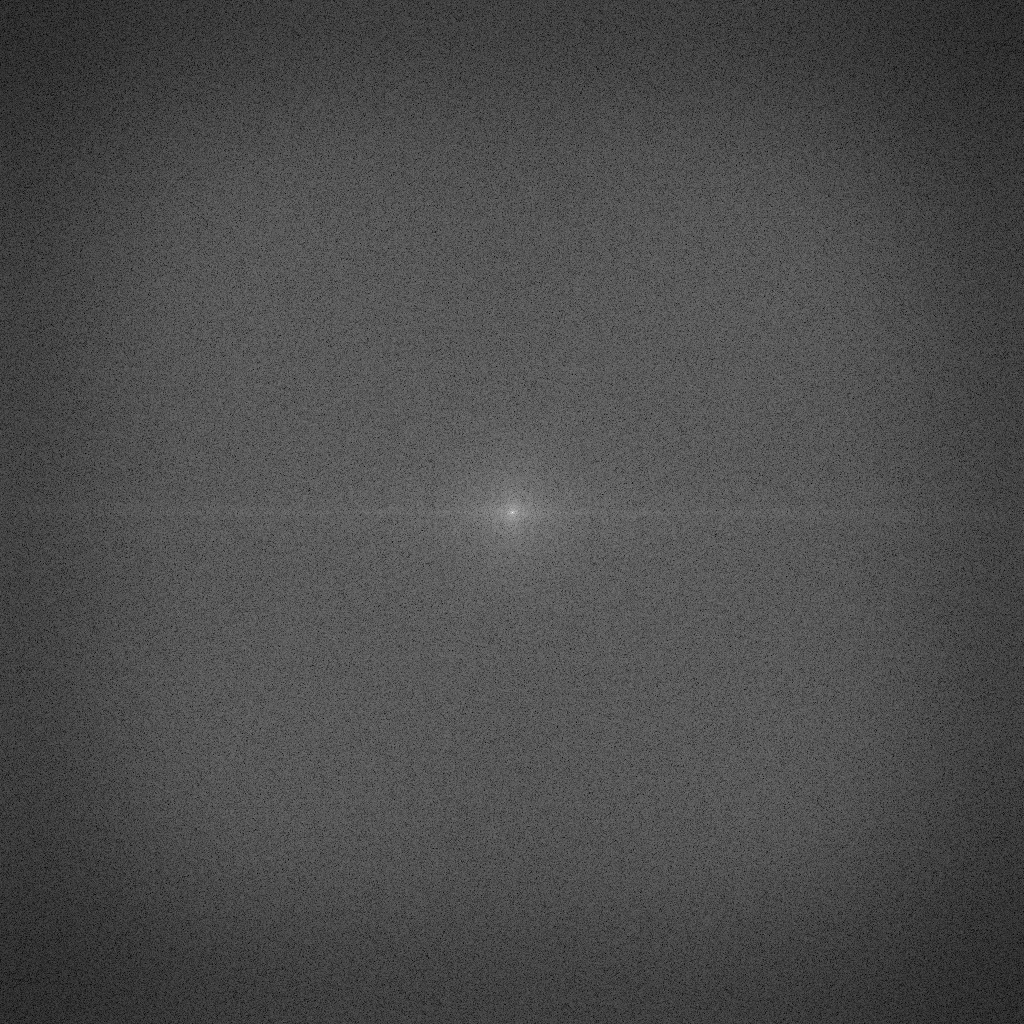
\includegraphics[width=0.16\textwidth]{img/ch6/dirty/fft6.png}

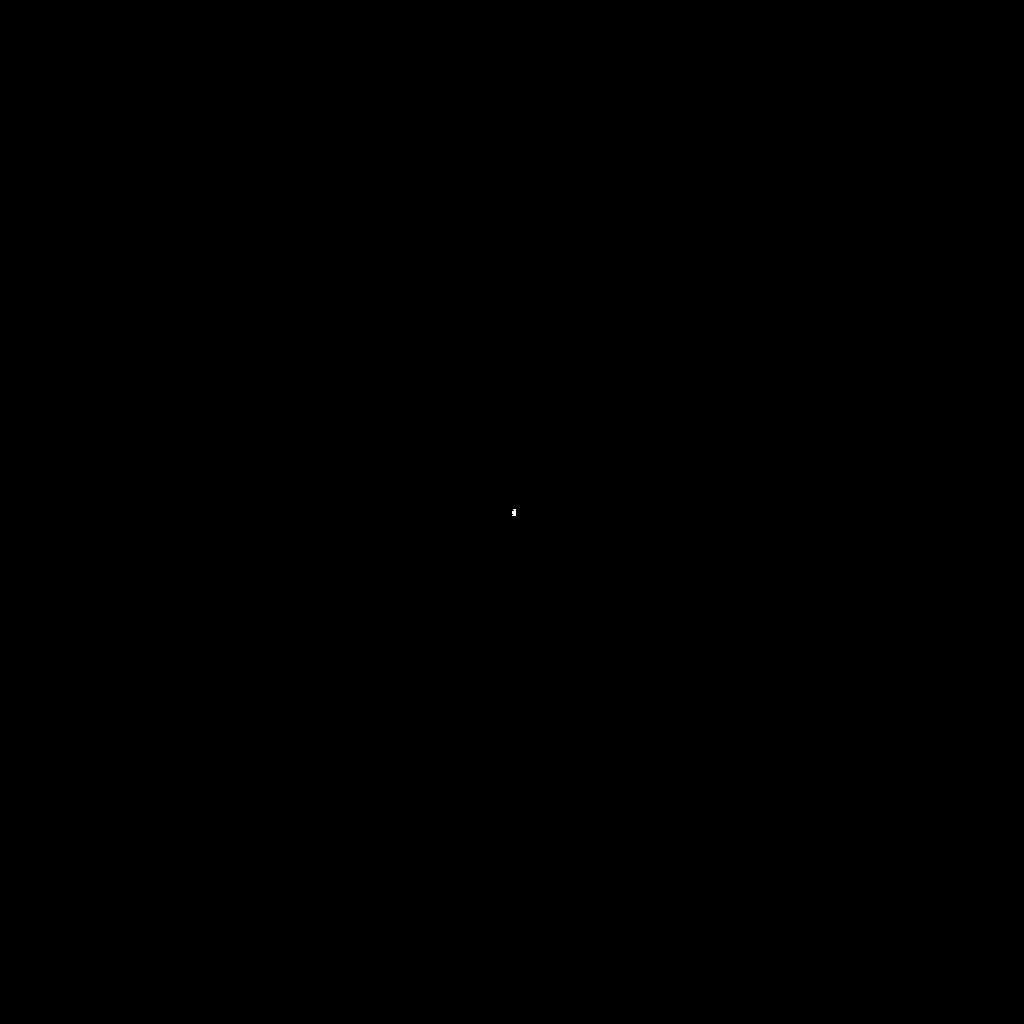
\includegraphics[width=0.16\textwidth]{img/ch6/dirty/freq1.png}
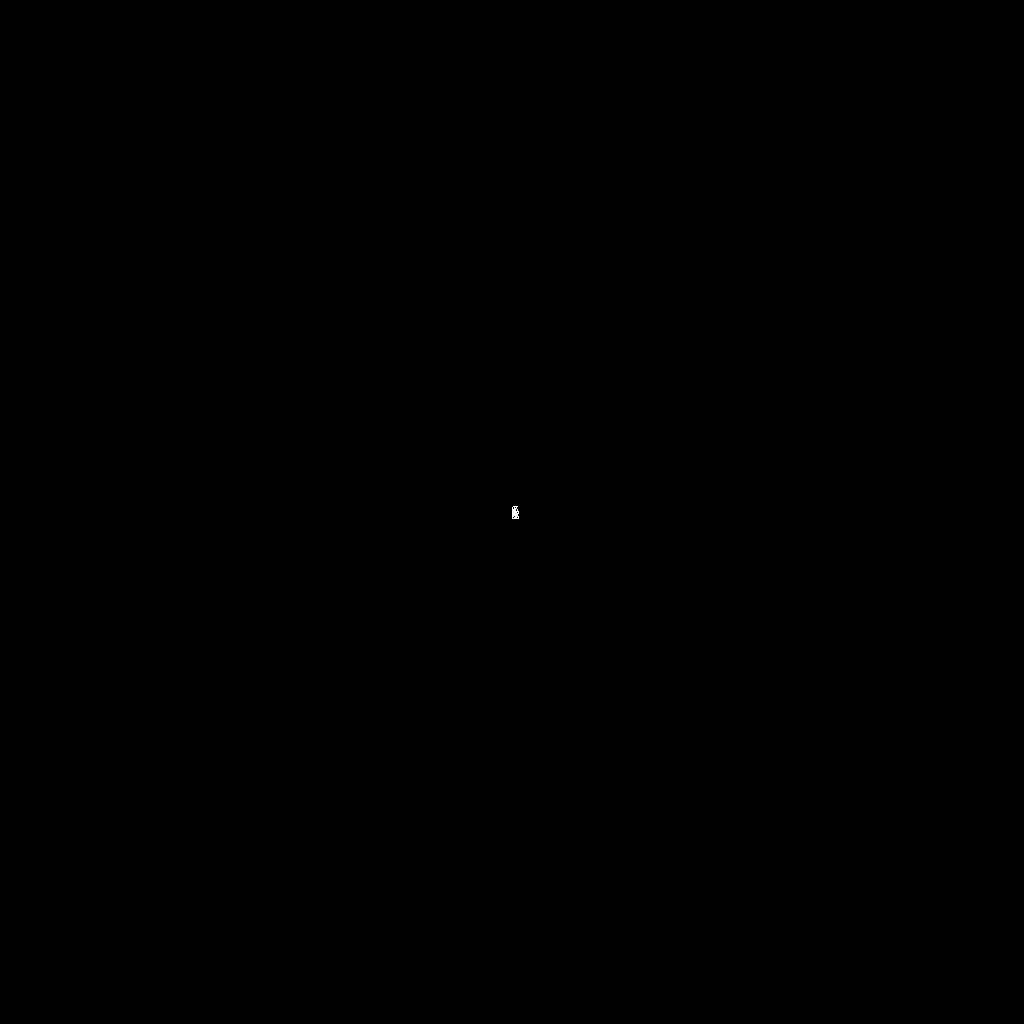
\includegraphics[width=0.16\textwidth]{img/ch6/dirty/freq2.png}
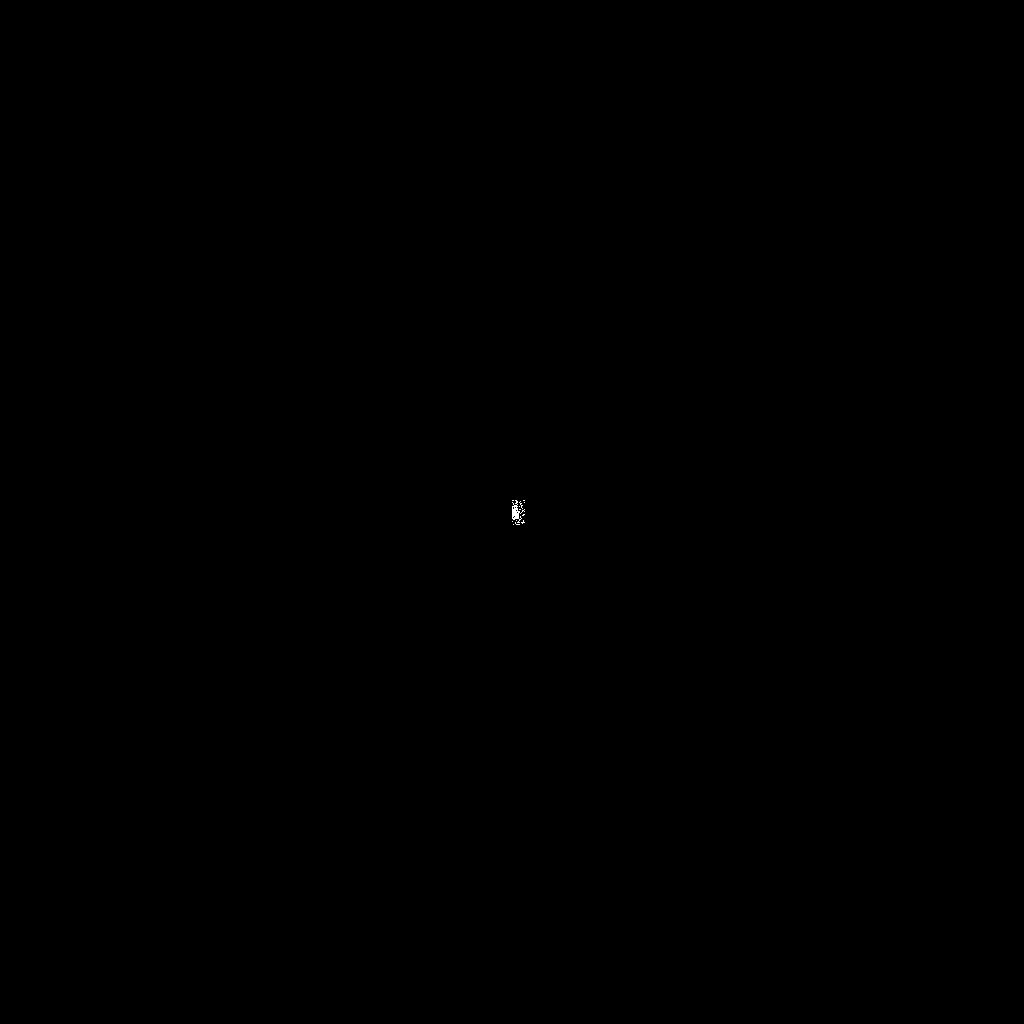
\includegraphics[width=0.16\textwidth]{img/ch6/dirty/freq3.png}
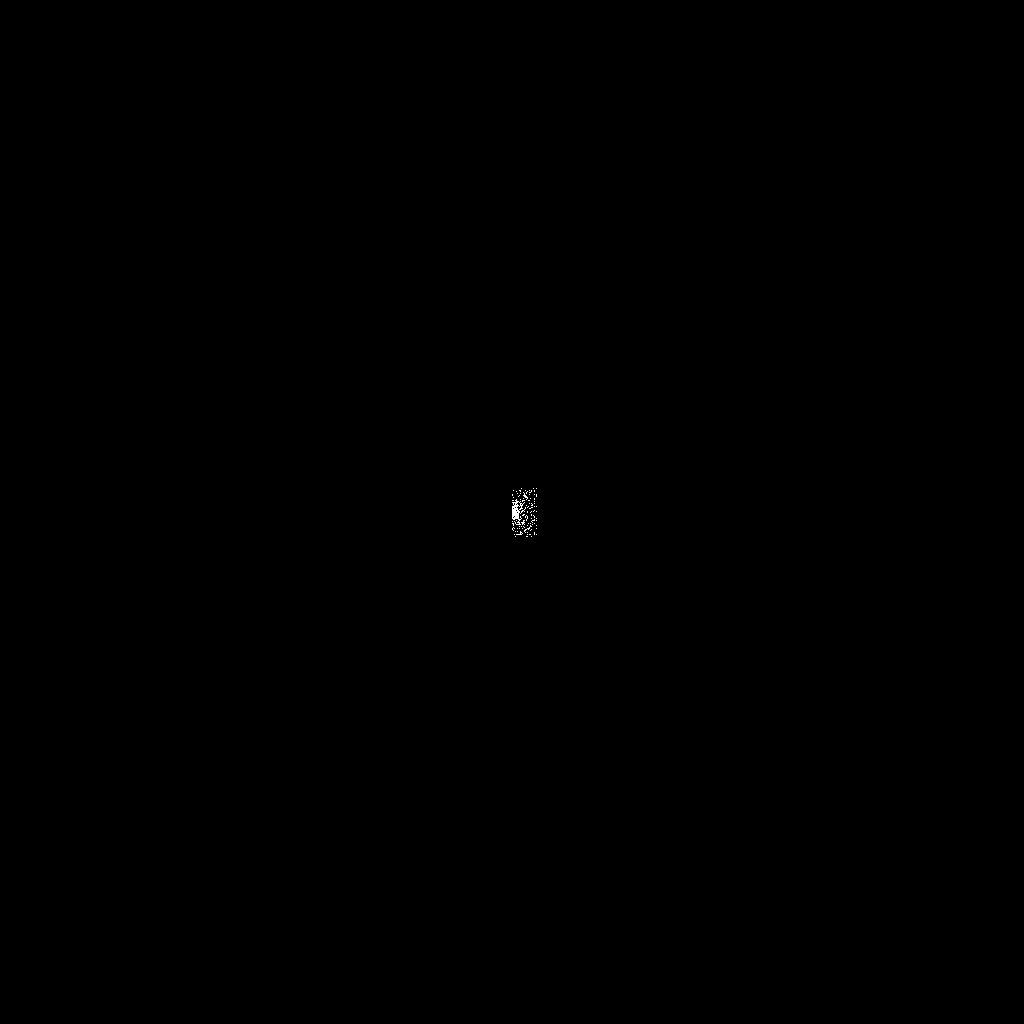
\includegraphics[width=0.16\textwidth]{img/ch6/dirty/freq4.png}
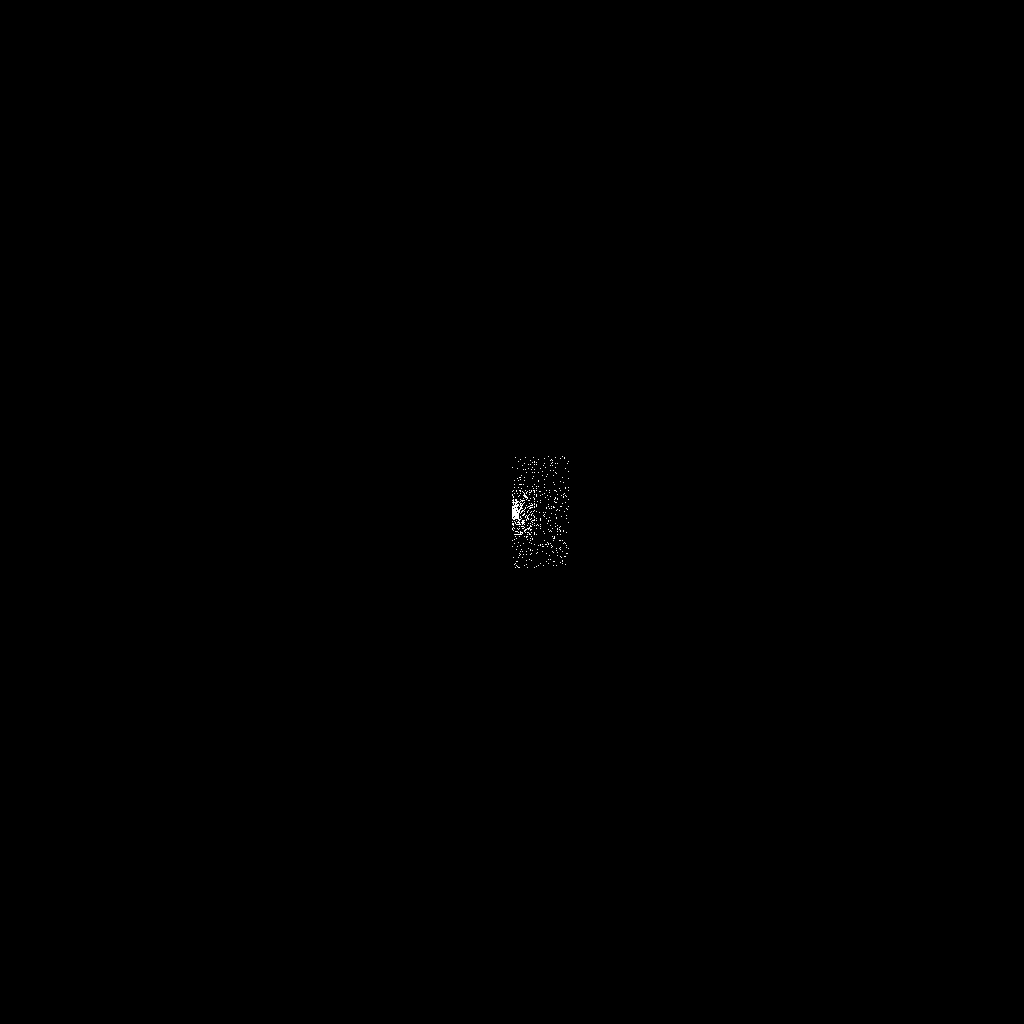
\includegraphics[width=0.16\textwidth]{img/ch6/dirty/freq5.png}
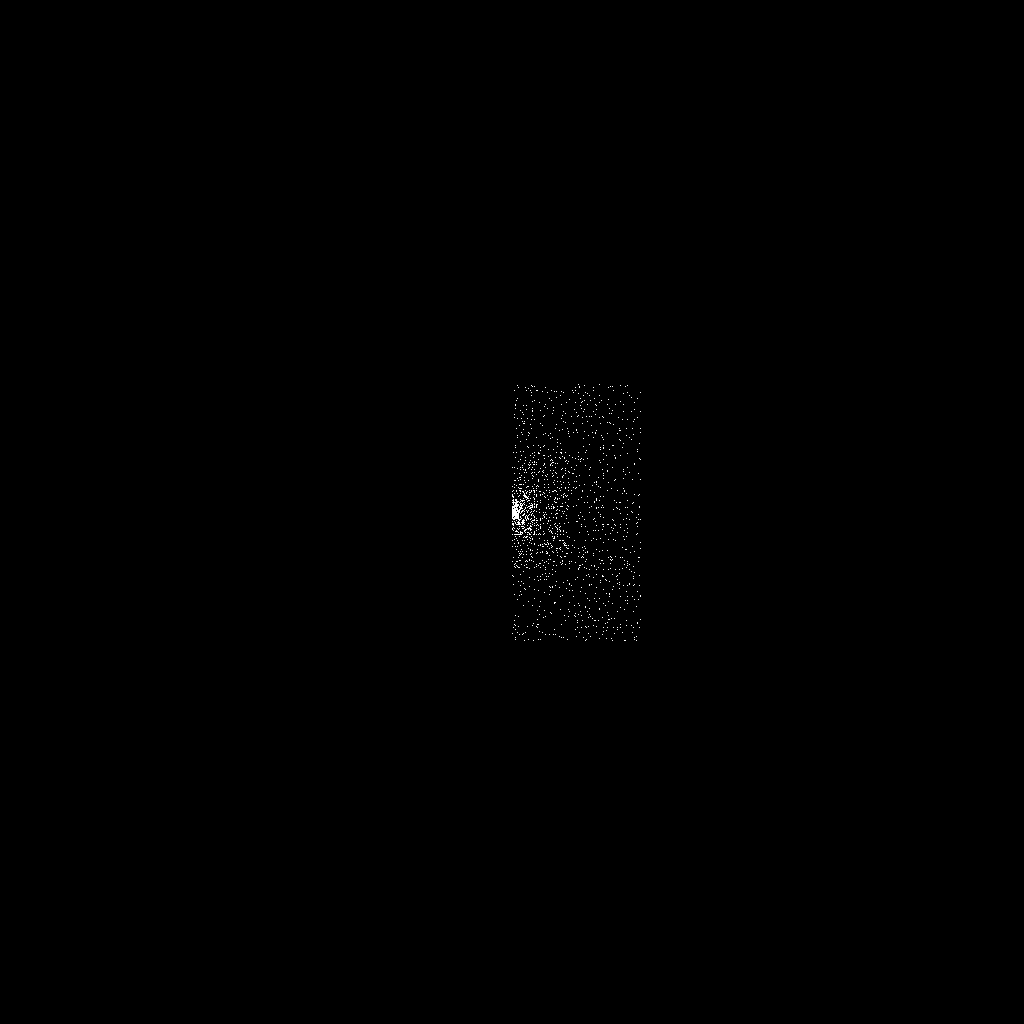
\includegraphics[width=0.16\textwidth]{img/ch6/dirty/freq6.png}

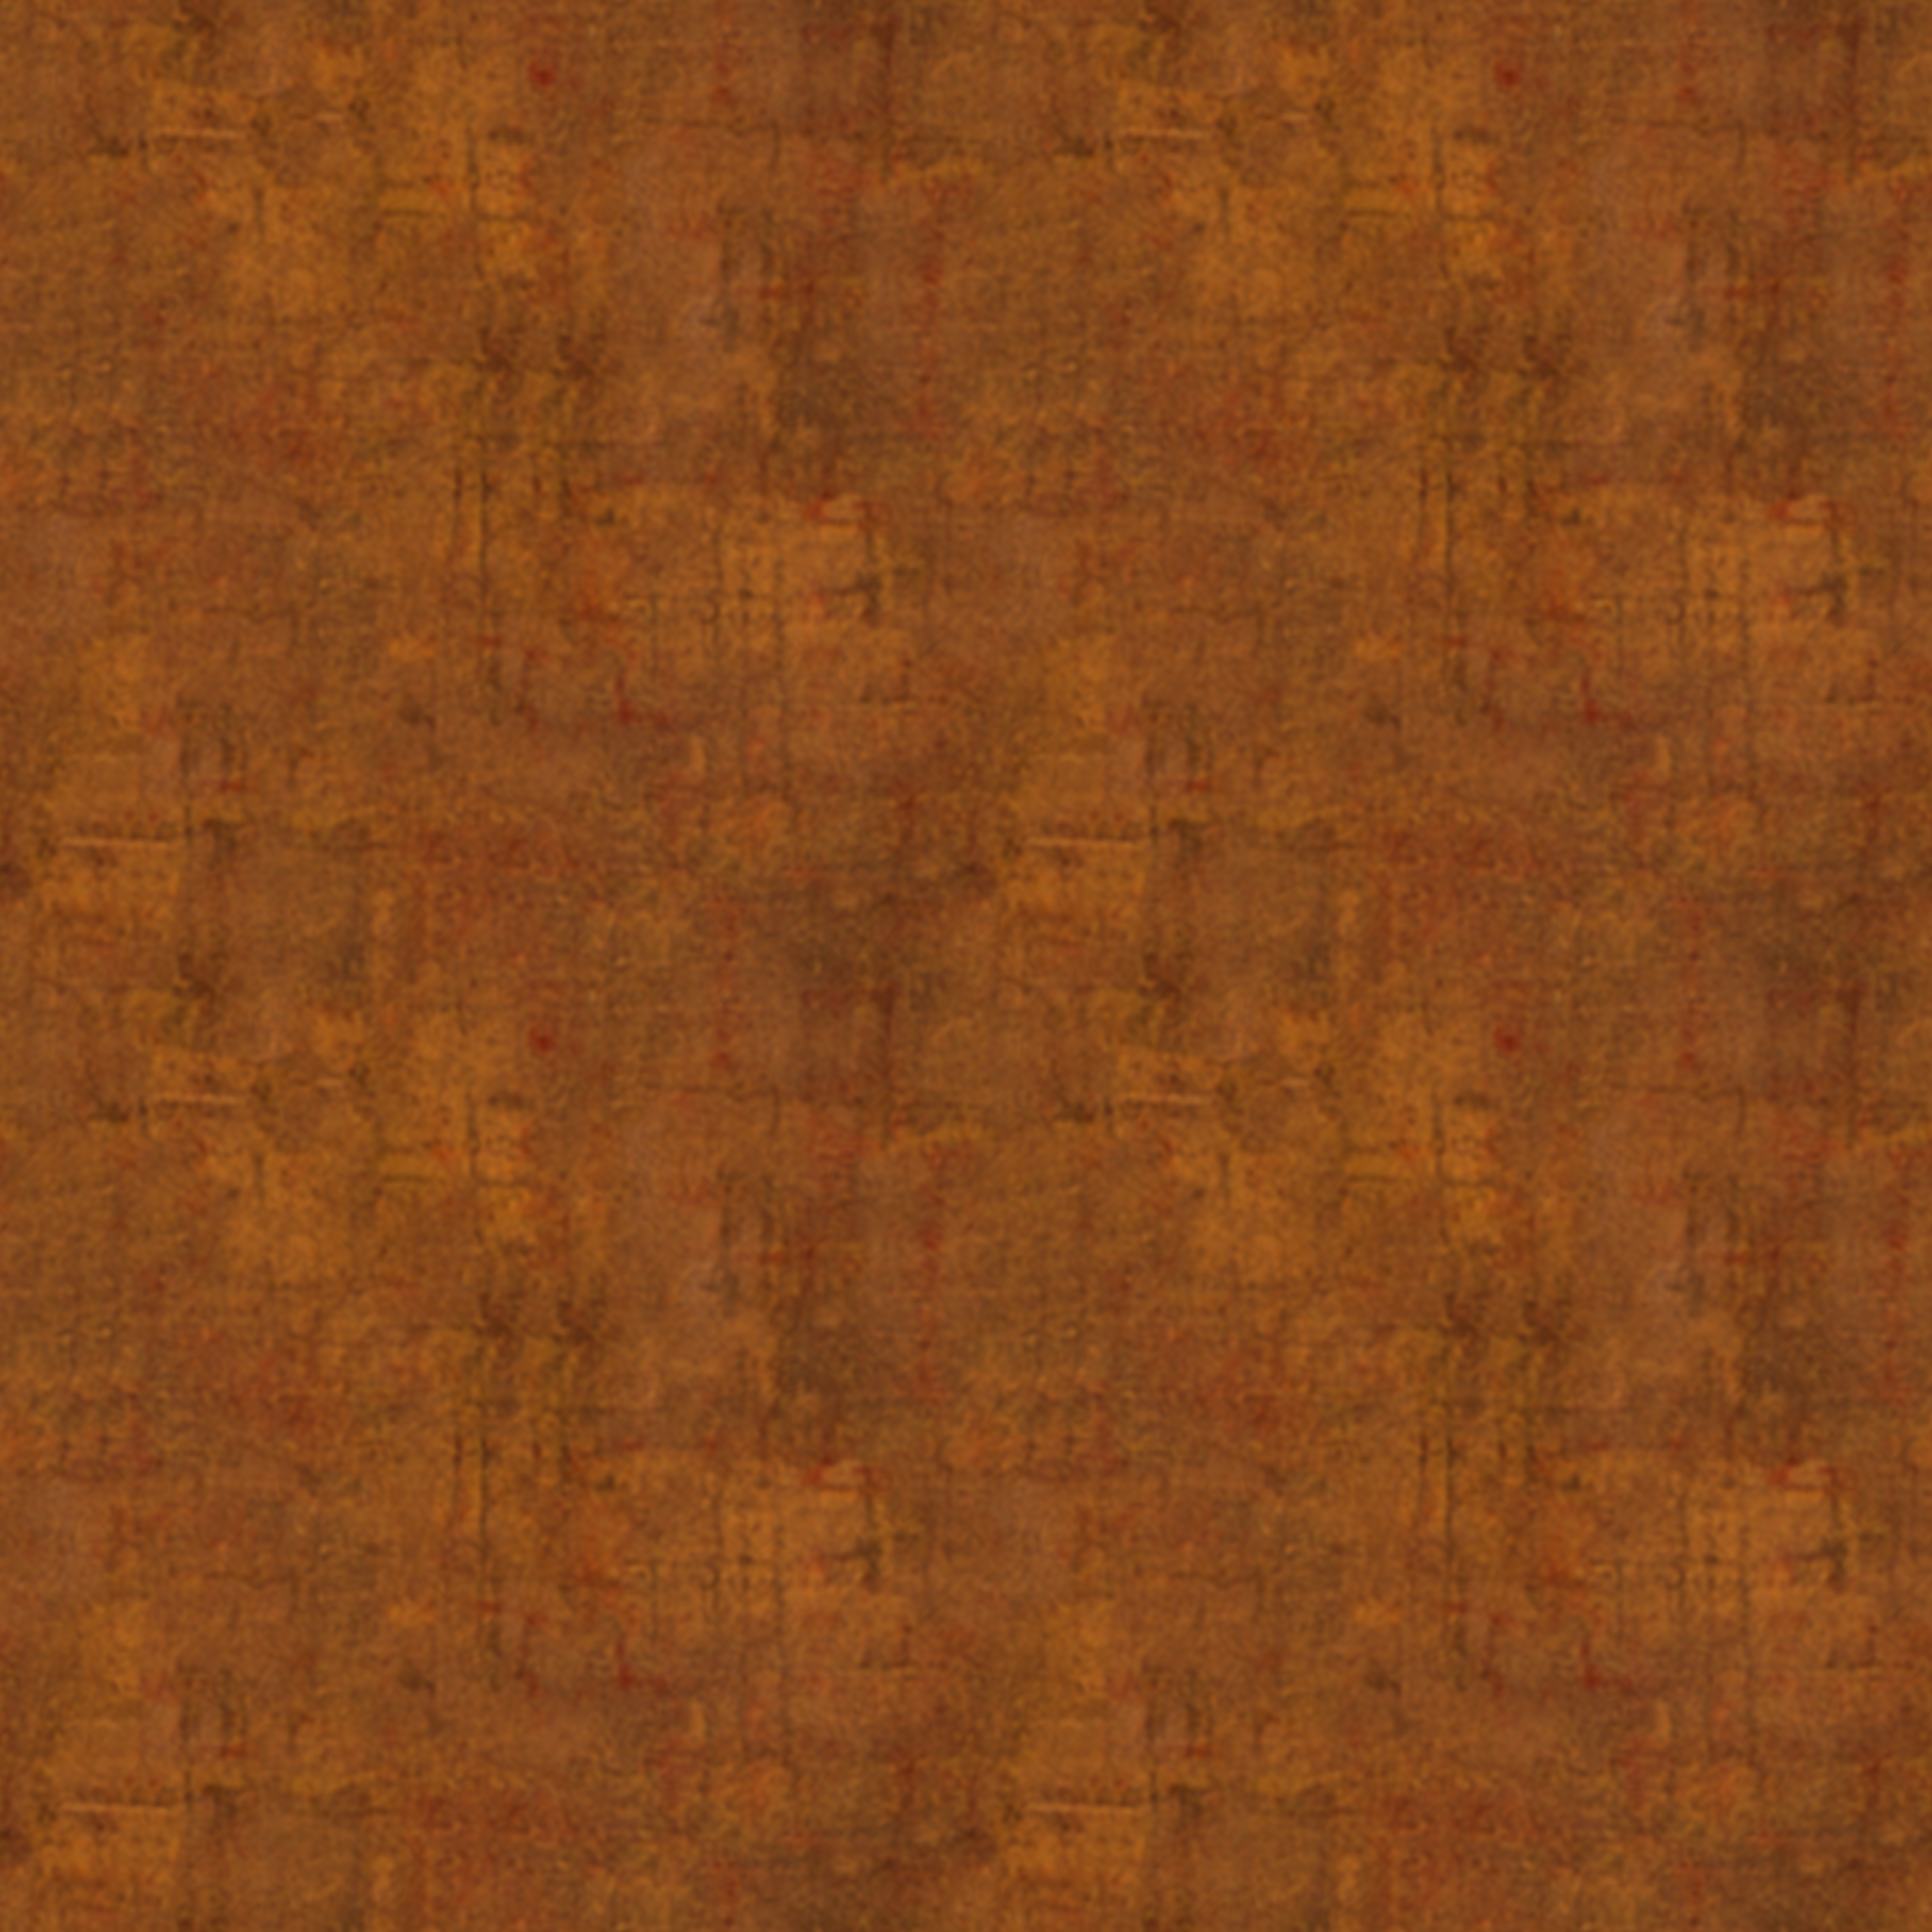
\includegraphics[width=0.325\textwidth]{img/ch6/dirty/ext4.png}
\includegraphics[width=0.324\textwidth]{img/ch6/dirty/ext5.png}
\includegraphics[width=0.325\textwidth]{img/ch6/dirty/ext6.png}
\caption{Dirty metal. 1st row: train data, the levels of the Gaussian pyramid from coarse to fine. 2nd row: Fast Fourier Transform (FFT) of the expanded pyramid level to the original resolution. 3rd row: all levels of a multiresolution model for the copper texture. 4th row: network inference Fourier spectra. 5th row: the cumulative selected frequencies for initialization of the first layer of each stage. 6th row: extrapolation of the periodic pattern at levels 4, 5, and 6.}
\label{f:dirty-extra}
\end{figure}


\begin{figure}[!h]
\centering

\includegraphics[width=0.16\textwidth]{img/ch6/copper/train1.png}
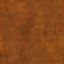
\includegraphics[width=0.16\textwidth]{img/ch6/copper/train2.png}
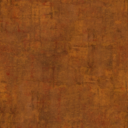
\includegraphics[width=0.16\textwidth]{img/ch6/copper/train3.png}
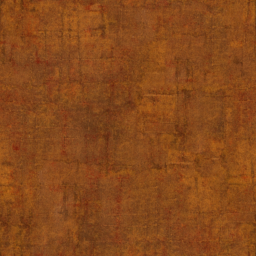
\includegraphics[width=0.16\textwidth]{img/ch6/copper/train4.png}
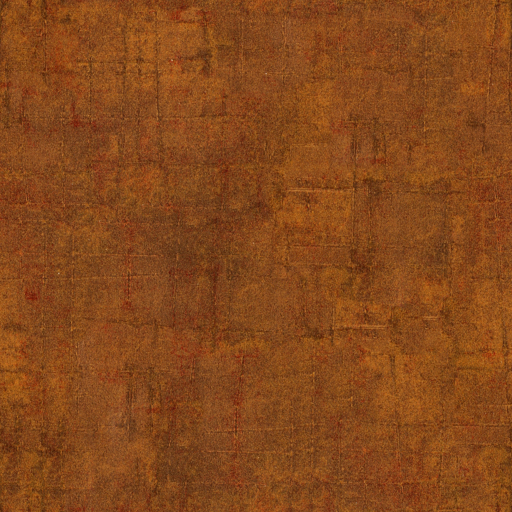
\includegraphics[width=0.16\textwidth]{img/ch6/copper/train5.png}
\includegraphics[width=0.16\textwidth]{img/ch6/copper/train6.png}

\includegraphics[width=0.16\textwidth]{img/ch6/copper/gfft1.png}
\includegraphics[width=0.16\textwidth]{img/ch6/copper/gfft2.png}
\includegraphics[width=0.16\textwidth]{img/ch6/copper/gfft3.png}
\includegraphics[width=0.16\textwidth]{img/ch6/copper/gfft4.png}
\includegraphics[width=0.16\textwidth]{img/ch6/copper/gfft5.png}
\includegraphics[width=0.16\textwidth]{img/ch6/copper/gfft6.png}

\includegraphics[width=0.16\textwidth]{img/ch6/copper/detail1.png}
\includegraphics[width=0.16\textwidth]{img/ch6/copper/detail2.png}
\includegraphics[width=0.16\textwidth]{img/ch6/copper/detail3.png}
\includegraphics[width=0.16\textwidth]{img/ch6/copper/detail4.png}
\includegraphics[width=0.16\textwidth]{img/ch6/copper/detail5.png}
\includegraphics[width=0.16\textwidth]{img/ch6/copper/detail6.png}

\includegraphics[width=0.16\textwidth]{img/ch6/copper/fft1.png}
\includegraphics[width=0.16\textwidth]{img/ch6/copper/fft2.png}
\includegraphics[width=0.16\textwidth]{img/ch6/copper/fft3.png}
\includegraphics[width=0.16\textwidth]{img/ch6/copper/fft4.png}
\includegraphics[width=0.16\textwidth]{img/ch6/copper/fft5.png}
\includegraphics[width=0.16\textwidth]{img/ch6/copper/fft6.png}

\includegraphics[width=0.16\textwidth]{img/ch6/copper/freq1.png}
\includegraphics[width=0.16\textwidth]{img/ch6/copper/freq2.png}
\includegraphics[width=0.16\textwidth]{img/ch6/copper/freq3.png}
\includegraphics[width=0.16\textwidth]{img/ch6/copper/freq4.png}
\includegraphics[width=0.16\textwidth]{img/ch6/copper/freq5.png}
\includegraphics[width=0.16\textwidth]{img/ch6/copper/freq6.png}

% \includegraphics[width=0.16\textwidth]{img/ch6/copper/ext1.png}
% \includegraphics[width=0.16\textwidth]{img/ch6/copper/ext2.png}
% \includegraphics[width=0.16\textwidth]{img/ch6/copper/ext3.png}
% \includegraphics[width=0.16\textwidth]{img/ch6/copper/ext4.png}
% \includegraphics[width=0.16\textwidth]{img/ch6/copper/ext5.png}
% \includegraphics[width=0.16\textwidth]{img/ch6/copper/ext6.png}

% \includegraphics[width=0.33\textwidth]{img/ch6/copper/ext1.png}
% \includegraphics[width=0.33\textwidth]{img/ch6/copper/ext2.png}
% \includegraphics[width=0.33\textwidth]{img/ch6/copper/ext3.png}
\includegraphics[width=0.325\textwidth]{img/ch6/copper/ext4.png}
\includegraphics[width=0.324\textwidth]{img/ch6/copper/ext5.png}
\includegraphics[width=0.325\textwidth]{img/ch6/copper/ext6.png}

%
\caption{Copper. 1st row: train data, the levels of the Gaussian pyramid from coarse to fine. 2nd row: Fast Fourier Transform (FFT) of the expanded pyramid level to the original resolution. 3rd row: all levels of a multiresolution model for the copper texture. 4th row: network inference Fourier spectra. 5th row: the cumulative selected frequencies for initialization of the first layer of each stage. 6th row: extrapolation of the periodic pattern at levels 4, 5, and 6.}
\label{f:copper-extra}
\end{figure}

\pagebreak

% % ---------------

\section{Seamlessness with Poisson Regularization}
\label{s:poisson-regularization}

When obtaining a sample for amaterial, the inherent irregulatiry in the pattern due to the cut, folding or illumination conditions often pose challenges when stitched together, resulting in visible seams. Achieving seamlessness in texture generation is crucial for many applications. To address this, we propose a novel loss function for training representational netwroks that enforces seamlessness using Poisson regularization. Our approach operates on the image gradients, enabling seamless reconstruction across tileable textures.

% Achieving seamlessness in texture generation is crucial for many applications, particularly when working with irregular material samples. These samples often pose challenges when stitched together, resulting in visible seams. 

% Let $\gt{f}: \Omega \subset \mathbb{R}^2 \to \mathcal{C}$ be an image, where $\Omega = [0, P_1] \times [0, P_2]$ represents a rectangular domain, and $\mathcal{C}$ the color space. We aim to approximate $\gt{f}$ using a periodic INR, $f: \mathbb{R}^2 \to \mathcal{C}$, with periods $(P_1, P_2)$, ensuring the resulting texture is seamless. To guarantee periodicity, we define the weights $\omega_{ij}$ in the first layer of $f$ as $k_{ij}\frac{2\pi}{P_i}$, where $k_{ij} \in \mathbb{Z}^2$. According to Theorem~\ref{t-periodic}, this setup ensures $f$ is periodic with periods $(P_1, P_2)$.

To enforce seamlessness at the boundary $\partial \Omega$, we design a loss function grounded in a variational Poisson problem. Specifically, we use the Jacobian, $\jac{\gt{f}}$, of the ground-truth image to train the periodic network $f$. We introduce a matrix field $U$ such that its primitive approximates a seamless texture at $\partial \Omega$. This is achieved by solving the following constrained minimization problem:

\begin{align}\label{e-gradient-interpolant}\small
\min \int_{\Omega} \lambda\norm{{\jac{f}-U}}^2dx \text{ subject to } (1-\lambda)(\gt{f}-f)=0 \text{ in } \Omega,
\end{align}

where $\lambda: \Omega \to [0,1]$ is a weight function. When $\lambda \approx 1$, the Jacobian of $f$ should match $U$, while for $\lambda \approx 0$, the condition $\gt{f} = f$ is enforced. Based on this, we propose the following loss function to train the parameters $\theta$ of $f$:

\begin{align}\label{e-blending-no-grad}\small
\mathscr{L}(\theta)={\int_{\Omega} \lambda\norm{{\jac{f}-U}}^2dx} + {\int_{\Omega} (1-\lambda)\big(\gt{f}-f\big)^2dx}.
\end{align}


This loss function effectively trains $f$ to "seamlessly clone" the primitive of $U$ within the domain $\Omega$. Unlike classical methods that rely on pixel manipulation \citep{perez2003}, our approach operates on the gradients of the image, allowing for smoother transitions and better flexibility. In particular, the mask $\lambda$ depends on the position $x$ and typically takes higher values near the boundary $\partial \Omega$, ensuring that the Jacobian matching occurs near the edges while the interior enforces color matching.

Moreover, since $f$ is periodic, we train it on the torus obtained by identifying opposite edges of $\Omega$. This way, we can "invert the notion of boundary condition", giving the value of the function, the color values, primarily at the interior of the image domain while the boundary is primarily supervised with the gradients. Classical methods do not offer such flexibility.

% we employ masks $\lambda$ to delineate the supervision of gradients at the border, while the color values are supervised within the interior of the region. 
% This allows for seamless tiling without the need for manual pixel adjustments, a key limitation of traditional approaches.
In practice, we employ a soft mask $\lambda$, computed via a distance function from the center of the region. While binary masks may yield acceptable results, they often introduce artifacts in the gradient field of the reconstructed texture (see Figure~\ref{f:training_masks}), necessitating manual adjustment of the loss function components. Soft masks, by contrast, provide smoother transitions and mitigate these issues.

\begin{figure}[h]
    \centering
    \includegraphics[width=0.80\textwidth]{img/ch6/gradients-merged.png}
    \caption{Binary mask (top), soft mask (bottom), and the normalized magnitude of the gradients of the respective trained networks. This is the gradient of the texture in the second column of Figure~\ref{f:seamless_examples}.}
    \label{f:training_masks}
\end{figure}

In Figure~\ref{f:seamless_examples}, we demonstrate the effectiveness of our method. The first row shows non-tileable materials, while the second row presents their seamless reconstructions. The first column illustrates a fabric sample with fine details, the second shows a pattern with medium geometric structures, and the third features a texture with larger details. Our method successfully conceals seams by evenly distributing photometric differences across the reconstructed textures, ensuring uniformity across the edges.

% \begin{figure}[!h]
% \centering
% \includegraphics[width=0.27\linewidth]{img/ch6/22fabric1.jpg}
% \includegraphics[width=0.27\linewidth]{img/ch6/22wall.jpg}
% \includegraphics[width=0.27\linewidth]{img/nch6/mosaic_leaves.jpg}\hfill\\
% \hspace{1pt}\includegraphics[width=0.27\linewidth]{img/ch6/extrapolation_jeans.png}
% \includegraphics[width=0.27\linewidth]{img/ch6/extrapolation_wall.png}
% \includegraphics[width=0.27\linewidth]{img/ch6/extrapolation-leaves.png}
% \caption{Seamless reconstruction of jeans fabric (fine details), a wall patch (medium details), and a leaf mosaic (larger details).}
% \label{f:seamless_examples}
% \end{figure}

\begin{figure}[h]
    \centering
    \begin{subfigure}[b]{0.32\textwidth}
        \centering
        \includegraphics[width=\textwidth]{img/ch6/22fabric1.jpg}
        % \caption{$\omega_0=2$ Hz}
        % \label{fig:pred-1hl-16hf-2hz}
    \end{subfigure}
    \begin{subfigure}[b]{0.32\textwidth}
        \centering
        \includegraphics[width=\textwidth]{img/ch6/22wall.jpg}
        % \caption{$\omega_0=4$ Hz}
        % \label{fig:16x-zoom-1hl-16hf-2hz}
    \end{subfigure}
    \begin{subfigure}[b]{0.32\textwidth}
        \centering
        \includegraphics[width=\textwidth]{img/ch6/mosaic_leaves.jpg}
        % \caption{$\omega_0=8$ Hz}
        % \label{fig:fft-1hl-16hf-2hz}
    \end{subfigure}

    \begin{subfigure}[b]{0.32\textwidth}
        \centering
        \includegraphics[width=\textwidth]{img/ch6/extrapolation_jeans.png}
        % \caption{$\omega_0=16$ Hz}
        % \label{fig:pred-1hl-256hf-2hz}
    \end{subfigure}
    \begin{subfigure}[b]{0.32\textwidth}
        \centering
        \includegraphics[width=\textwidth]{img/ch6/extrapolation_wall.png}
        % \caption{$\omega_0=32$ Hz}
        % \label{fig:16x-zoom-1hl-256hf-2hz}
    \end{subfigure}
    \begin{subfigure}[b]{0.32\textwidth}
        \centering
        \includegraphics[width=\textwidth]{img/ch6/extrapolation-leaves.png}
        % \caption{$\omega_0=64$ Hz}
        % \label{fig:pred-1hl-16hf-64hz}
    \end{subfigure}
    \caption{Seamless reconstruction of jeans fabric (fine details), a wall patch (medium details), and a leaf mosaic (larger details).}
    \label{f:seamless_examples}
\end{figure}


% \section{Training Seamless with Poisson Regularization}
% \label{s-training}

% Let $\gt{f}:\Omega\subset\R^2\to \mathcal{C}$ be an image (\textit{ground-truth}) defined in the rectangular domain $\Omega=[0,P_1]\times[0,P_2]$. 
% We aim to approximate $\gt{f}$ by a periodic INR ${f}:\R^2\to \mathcal{C}$ with periods $(P_1, P_2)$ such that the resulting image is seamless. 
% For this, define the weights $\omega_{ij}$ of the first layer of $f$ in the form $k_{ij}\frac{2\pi}{P_i}$ with $k_{ij}\in \Z^2$.
% Again, this implies that the first layer is periodic with periods $(P_1,P_2)$, then, Theorem~\ref{t-periodic} implies that $f$ is also periodic with the same periods. 
% To force the resulting texture to be seamless at the boundary $\partial \Omega$ of $\Omega$, we design a loss function based on a \textit{Poisson problem}.


% Specifically, we use the Jacobian $\jac{\gt{f}}$ of $\gt{f}$ to train the periodic INR $f$.
% For this, we define a matrix field $U$ such that its primitive approximates a seamless tileable texture at $\partial \Omega$.
% % %
% Then we enforce $\gt{f}=f$ at some region of $\Omega$. This can be modeled using:
% \begin{align}\label{e-gradient-interpolant}\small
% \min \int_{\Omega} \lambda\norm{{\jac{f}-U}}^2dx \text{ subject to } (1-\lambda)(\gt{f}-f)=0 \text{ in } \Omega.
% \end{align}
% Where $\lambda:\Omega\to [0,1]$ is a weight function indicating that $U$ should match the Jacobian of $f$ if it is close to one ($\lambda\approx 1$), and enforces $\gt{f}=f$, otherwise. 
%  We propose to use this variational problem to define the following loss function to train the parameters $\theta$ of $f$.
% \begin{align}\label{e-blending-no-grad}\small
% \mathscr{L}(\theta)={\int_{\Omega} \lambda\norm{{\jac{f}-U}}^2dx} + {\int_{\Omega} (1-\lambda)\big(\gt{f}-f\big)^2dx}.
% \end{align}
% \noindent
% Thus, $\mathscr{L}$ trains $f$ to \textit{seamless clone} the primitive of $U$ to $f$ in $\Omega$.
% Unlike classical approaches that rely on pixel manipulation, seamless cloning operates on the image gradients.
% Note that $\lambda$ depends on the position $x$. In practice, we consider it to have high values near $\partial \Omega$. As a result, the training forces the matching of the Jacobian of $f$ with $U$ near $\partial \Omega$. In fact, since $f$ is periodic, we are training it on the torus given by the identification of the opposite edges of $\Omega$.
% Classical methods do not provide such flexibility.

% \section{Experiments}

% This section details experiments carried out using our method to represent tileable material textures. We begin by fitting a tileable pattern across different scales and evaluate its performance qualitatively. Next, we train the network on a sample containing repetitions of the pattern, where the fundamental period is smaller than the training domain. Our goal is to examine how the choice of the network's period influences pattern reconstruction. Additionally, we use masks during training to selectively exclude specific image regions, testing the network's accuracy in reconstructing them.

% Moreover, we address non-tileable patterns that we make seamless using our Poisson regularization technique. Lastly, we provide comparative evaluations with established methods in the field.

% \subsection{Seamless Tileable Materials}\label{s-multires-2d}

% We start with a single tile, matching the fundamental period of a texture, with a resolution of $512^2$ pixels and $8$ bits per color channel in \texttt{RGB} space. The network is trained in the domain $[-1, 1] \times [-1, 1]$ and, thus, we set its period as $2$. The initialization uses the scheme described in Sec~\ref{s-initialization} \red{with the maximum frequency} $\omega=32$. \red{Table XXX} displays the architecture of the network used in this experiment, while Figure \ref{f:periodic-reconstruction} shows the ground truth image, the result of the reconstruction in the training domain and the exptrapolation in the domain [-2, 2]. Observe that the ground truth image and the reconstructed image exhibit a high degree of similarity with a \red{PSNR of XX.X dB}.


% \begin{figure}
%     \centering
%     \begin{subfigure}[b]{0.3\textwidth}
%         \centering
%         \includegraphics[width=\textwidth]{img/placeholder512.png}
%         \caption{$Ground truth$}
%         \label{fig:y equals x}
%     \end{subfigure}
%     \hfill
%     \begin{subfigure}[b]{0.3\textwidth}
%         \centering
%         \includegraphics[width=\textwidth]{img/placeholder512.png}
%         \caption{Reconstruction in $[-1, 1]$}
%         \label{fig:three sin x}
%     \end{subfigure}
%     \hfill
%     \begin{subfigure}[b]{0.3\textwidth}
%         \centering
%         \includegraphics[width=\textwidth]{img/placeholder512.png}
%         \caption{Extrapolation in $[-2, 2]$}
%         \label{fig:five over x}
%     \end{subfigure}
%        \caption{Reconstruction using periodic network}
%        \label{f:periodic-reconstruction}
% \end{figure}

% Figure \ref{f:comparison-siren} illustrates a comparison between training a neural network initialized with our method against training a network initialized as Siren. Note that without our periodic initialization, the network only learns the periodic tile inside the domain of supervision, exhibiting noise when evaluated in another set of coordinates.

% \begin{figure}
%     \centering
%     \begin{subfigure}[b]{0.24\textwidth}
%         \centering
%         \includegraphics[width=\textwidth]{img/ch6/mnet_extrapolation.png}
%         \caption{Ours in $[-2, 2]^2$}
%         \label{f:periodic-leopard-regular}
%     \end{subfigure}
%     % \hfill
%     \begin{subfigure}[b]{0.24\textwidth}
%         \centering
%         \includegraphics[width=\textwidth]{img/ch6/siren_extrapolation.png}
%         \caption{Siren in $[-2, 2]^2$}
%         \label{f:siren-leopard-regular}
%     \end{subfigure}
%     \begin{subfigure}[b]{0.24\textwidth}
%         \centering
%         \includegraphics[width=\textwidth]{img/ch6/siren_extrapolation.png}
%         \caption{Ours in $[-9, -6] \times [1, 4]$}
%         \label{f:periodic-leopard-translated}
%     \end{subfigure}
%     \begin{subfigure}[b]{0.24\textwidth}
%         \centering
%         \includegraphics[width=\textwidth]{img/ch6/siren_extrapolation.png}
%         \caption{Siren in $[-9, -6] \times [1, 4]$}
%         \label{f:siren-leopard-translated}
%     \end{subfigure}
%        \caption{Our periodic network vs Siren}
%        \label{f:comparison-siren}
% \end{figure}

% As we've demonstrated in chapter \ref{ch:mrnet}, the networks of the MR-Net family are analytically equivalent to a deep sinusoidal neural network. This way it is expected that this periodic initialization also works in multiresolution. To validate this hypothesis, we train a M-Net model, using the framework described in \ref{ch:mrnet}, consisting of $6$ stages. The architecture of the hidden layer (number of input/output neurons) and the band limits of the first layer for each stage are in Table \ref{tab:mnet-architecture}.

% \begin{table}[h]
% \small
% \begin{tabular}{|l|c|l|l|}
% \hline
% \textbf{Stage} & \multicolumn{1}{l|}{\textbf{Band-Limit}} & \multicolumn{1}{l|}{\textbf{Hidden Input}} & \multicolumn{1}{l|}{\textbf{Hidden Output}} \\ \hline
%  0     & $[0, 3]\times[-3, 3]$                       & 24                                & 32                                 \\
%  1     & $[0, 6]\times[-6, 6]$                       & 48                                & 32                                 \\
%  2     & $[0, 12]\times[-12, 12]$                     & 80                                & 64                                 \\
%  3     & $[0, 24]\times[-24, 24]$                     & 192                               & 160                                \\
%  4     & $[0, 56]\times[-56, 56]$                     & 384                               & 256                                \\
%  5     & $[0, 128]\times[-128, 128]$                   & 1024                              & 512                                \\ \hline
% \end{tabular}
% \caption{M-Net architecture.}
% \end{table}\label{tab:mnet-architecture}


% Figure \ref{f:rec_gt} presents a qualitative comparison between the original image and the reconstructed image at the finest scale. Once again, our method achieves a high-quality reconstruction with a \red{PNSR of XX.X db}. Additionally, our model achieves this level of fidelity using 855,572 parameters, which is less than the number of pixels in the image ($1024^2 = 1,048,576$). 

% \red{Our model also demonstrated the ability to encode information at multiresolution giving an even better compression compared to a traditional Mipmap. [What is the size of each file? Can I zip the network weights?]}

% \begin{figure}[h]
% \centering
% \includegraphics[width=0.42\linewidth]{img/placeholder512.png}
% \includegraphics[width=0.42\linewidth]{img/placeholder512.png}
% \caption{Original image (left); reconstruction of the network (right) 
% }
% \label{f:rec_gt}
% \end{figure}

% To verify the periodicity of our model, we evaluate the network in a larger domain ($[-2, 2]^2$) than its training domain $[-1, 1]^2$; Figure~\ref{f:mr-periodic} illustrates it for levels of detail 2, 4, and 6.

% \begin{figure}[!h]
% \centering
% \includegraphics[width=0.84\linewidth]{img/placeholder512.png}
% \caption{Reconstructed multiresolution levels extrapolation. Top left: level 2; bottom left: level 4; right: level 6.}
% \label{f:mr-periodic}
% \end{figure}

% \subsection{Repeating Patterns in Sample}

% We can also represent a texture with a fundamental period smaller than the sample size. 
% This means that the periodic pattern repeats multiple times within the sample. 
% To address this, we can specify the fundamental period either by prior knowledge or through pre-processing of the image, and train the network using the entire data or only a specific portion of it.

% Figure \ref{f:mask_nomask} showcases a texture sample where the pattern is repeated twice, and its extrapolated reconstructions in the region $[0, 3]^2$. The training considered $[-1, 1]^2$, with a specified period of 1. Figures~\ref{f:mask_nomask} (a) and (c) show the training data, while the network reconstruction is given by (b) and (d), respectively. 
% In (a-b), all coordinates within the region are provided, thus the network learns a periodic representation of the pattern. 
% In (c-d), we employ a mask to exclude a small part while preserving a contiguous region that contains the fundamental period. Again, our method reconstructs the periodic pattern across the entire region. This demonstrates that the over-determined problem does not negatively impact the results. 

% \begin{figure}[!h]
% \centering
% \includegraphics[width=0.24\linewidth]{img/victorian/tile_vitorian.png}
% \includegraphics[width=0.24\linewidth]{img/victorian/extrapolation_nomask.png}
% \includegraphics[width=0.24\linewidth]{img/victorian/train-crab.png}
% \includegraphics[width=0.24\linewidth]{img/victorian/extrapolation-crab.png}
% % \includegraphics[width=0.24\linewidth]{img/victorian/train-face.png}
% % \includegraphics[width=0.24\linewidth]{img/victorian/train-face-mid.png}
% % \includegraphics[width=0.24\linewidth]{img/victorian/extrapolation-face.png}
% % \includegraphics[width=0.24\linewidth]{img/victorian/extrapolation-face-mid.png}
% \vspace{-0.2cm}
% % \includegraphics[width=0.48\linewidth]{img/stochastic_mask.png}
% % \includegraphics[width=0.48\linewidth]{img/extrapolation_randommask.png}
% \centerline{(a)\hfil\hfil(b)\hfil\hfil(c)\hfil\hfil(d)}
% \vspace{-0.4cm}
% \caption{(a) Full training data. (b) Network reconstruction from full data. (c) Masked training data; black pixels were not provided in training. (d) Network reconstruction from masked data.}
% \label{f:mask_nomask}
% \end{figure}

% In the next experiment, a few points have no correspondents visible in any of the periods. This generates an artifact that is noticed across all occurrences of that pattern (Figure \ref{f:artifact}).

% \begin{figure}[!h]
% \centering
% \includegraphics[width=0.27\linewidth]{img/victorian/train-face-mid.png}
% \includegraphics[width=0.27\linewidth]{img/victorian/extrapolation-face-mid.png}
% \includegraphics[width=0.27\linewidth]{img/victorian/artifact.png}
% \vspace{-0.4cm}
% \caption{From left to right: training data, network reconstruction in $[0, 3]^2$, and zoom in one tile to highlight the reconstruction artifact.}
% \label{f:artifact}
% \end{figure}


% Next, we selectively remove points from the training data encouraging a sparse representation of the pattern. We generate the mask by randomly selecting a pixel and subsequently discarding all pixels that correspond to the selected one based on the pattern's period. 
% These steps are repeated until no additional pixels remain to be sampled. 
% Consequently, the mask encompasses exactly $1/4$ of the total pixels. Figure \ref{f:masked_recontruction} shows the training data, where the black pixels were removed from training, and the learned texture in $[2, 6]^2$. 

% \begin{figure}[!h]
% \centering
% \includegraphics[width=0.4\linewidth]{img/ch6/stochastic_mask.png}
% \includegraphics[width=0.4\linewidth]{img/ch6/extrapolation_randommask.png}
% \caption{On the left, the masked input data, where the black pixels were removed from training. On the right, the network reconstruction.~\\
% }
% \label{f:masked_recontruction}
% \end{figure}

% Even in this case, our method captures the underlying periodicity. This provides evidence that we can use the training data at any part of the domain. In other words, we only need a single sample from the class of equivalence defined by the periodicity to reconstruct the image without requiring any additional regularization.

% \subsection{Seamless with Poisson Regularization}\label{s:poisson-regularization}

% When obtaining a sample for a material, the inherent irregularity in the sample's pattern poses a challenge in seamlessly stitching it together. Achieving a seamless material is crucial for numerous applications. This section details the application of our methodology to generate seamless results from material patches.

% We train a periodic INR for this task using the loss function of Section~\ref{s-training} which is based on the Poisson equation. In regard to classical Poisson problem solutions, a key observation of our method is the inversion of boundary and interior conditions. 
% We employ masks (the function $\lambda$ in Eq~\ref{e-blending-no-grad}) to delineate the supervision of gradients at the border, while color values are supervised within the interior of the region. Given that our work is situated in the realm of periodic functions, the problem domain is equivalently represented as a torus, thus obviating traditional boundaries.


% While binary masks can produce satisfactory outcomes, they often introduce artifacts at the gradient of the reconstructed network (Figure \ref{f:training_masks}), requiring customized adjusts, per image, of the weights of the loss function components. Consequently, we opted for soft masks computed via a distance function to the center of the mask. 
% In our experiments, we utilized the $L_2$ distance, but any $L_p$ distance can be employed as a parameter for refining the results. 
% \begin{figure}[!h]
% \centering
% \includegraphics[width=0.90\linewidth]{img/placeholder512.png}
% % \includegraphics[width=0.32\linewidth]{img/non-tileable/hard_mask_d0.png}
% % \includegraphics[width=0.32\linewidth]{img/non-tileable/soft_mask_d0.png}

% % \includegraphics[width=0.32\linewidth]{img/non-tileable/hard_gradient.png}
% % \includegraphics[width=0.32\linewidth]{img/non-tileable/soft_gradient.png}

% \caption{Binary mask (top), soft mask (bottom), and the normalized magnitude of the gradients of the trained networks. This is the gradient of the texture in Line 2 of Fig \ref{f:seamless_examples}.}
% \label{f:training_masks}
% \end{figure}


% \begin{figure}[!h]
% \centering
% \includegraphics[width=0.40\linewidth]{img/non-tileable/22fabric1.jpg}
% \includegraphics[width=0.40\linewidth]{img/non-tileable/extrapolation_jeans.png}
% \vspace{-0.2cm}
% \caption{Seamless reconstruction of jeans fabric}
% \label{f:extrapolation_jeans}
% \end{figure}

% \begin{figure}[!h]
% \centering
% \includegraphics[width=0.38\linewidth]{img/non-tileable/mosaic_leaves.jpg}
% % \includegraphics[width=0.20\linewidth]{img/non-tileable/mask_d1.png}
% % \includegraphics[width=0.20\linewidth]{img/non-tileable/mask_d1.png}
% \includegraphics[width=0.38\linewidth]{img/non-tileable/extrapolation-leaves.png}

% \caption{Wonderful caption}
% \label{f:seamless_reconstruction}
% \end{figure}

% Figure~\ref{f:seamless_examples} illustrates several seamless reconstructions (second column) of non-tileable material samples (first column).
% The first line shows an example of a fabric patch containing only fine details.
% The second line gives the case of a pattern featuring medium geometric details. Meanwhile, the third line presents the reconstruction of a pattern characterized by larger details. 
% Note that in all instances, our method adeptly conceals seams through the uniformization of photometric discrepancies. 
% This results in a visually cohesive representation that effectively camouflages the transitions between material patches.
% \begin{figure}[!h]
% \centering
% \includegraphics[width=0.43\linewidth]{img/non-tileable/22fabric1.jpg}
% \includegraphics[width=0.43\linewidth]{img/non-tileable/extrapolation_jeans.png}
% \includegraphics[width=0.43\linewidth]{img/non-tileable/22wall.jpg}
% \includegraphics[width=0.43\linewidth]{img/non-tileable/extrapolation_wall.png}
% \includegraphics[width=0.43\linewidth]{img/non-tileable/mosaic_leaves.jpg}
% \includegraphics[width=0.43\linewidth]{img/non-tileable/extrapolation-leaves.png}
% \vspace{-0.4cm}
% \caption{Seamless reconstruction of jeans fabric (only fine details), a patch of a wall (medium details). Note that although this texture looks homogeneous it has fine details as can be seen on its gradient in Fig ~\ref{f:training_masks}. Finally, the third line gives the reconstruction of the leaves textures containing big details.
% }
% \label{f:seamless_examples}
% \end{figure}

% % \begin{figure}[!h]
% % \centering
% % \includegraphics[width=0.40\linewidth]{img/non-tileable/22wall.jpg}
% % \includegraphics[width=0.40\linewidth]{img/non-tileable/extrapolation_wall.png}
% % \vspace{-0.2cm}
% % \caption{Material patch of a wall with intricate details. Note that although this texture looks very homogeneous it has fine details as can be seen on its gradient is on Fig 6.}
% % \label{f:seamless_wall}
% % \end{figure}

% % \vspace{-0.6cm}

% % \begin{figure}[!h]
% % \centering
% % \includegraphics[width=0.40\linewidth]{img/non-tileable/mosaic_leaves.jpg}
% % \includegraphics[width=0.40\linewidth]{img/non-tileable/extrapolation-leaves.png}
% % \vspace{-0.2cm}
% % \caption{Texture with big details}
% % \label{f:seamless_leaves}
% % \end{figure}


% % \subsection{Incremental and Compatible Materials}

% % \lnote{red}{
% % Se possivel Fazer o experimento e escrever a seção.
% % dar exemplos de incremental material / compatible material
% % }

\section{Comparisons}

% Here we show that employing periodic activation functions is insufficient for learning periodic images with supervision in a restricted domain. Figure \ref{f:siren-comparison} shows a comparison between image reconstruction/extrapolation using Siren's initialization and our periodic initialization. In this comparison, we use an identical architecture to SIREN: periodic INR with 3 hidden layers, of the form $\R^{256}\to \R^{256}$. The key difference lies in the initialization: we randomly selected 256 pairs of integer frequencies from the range $[0, 30]\times[-30, 30]$, whereas SIREN follows the initialization given in \cite{sitzmann2019siren} with $\omega_0=30$. The images were trained on a $512\times512$ grid within the region $[-1, 1]$ for 500 epochs. The extrapolations are displayed in the interval $[-2, 2]$.

First, we demonstrate that employing periodic activation functions alone is insufficient for learning periodic images with supervision over a restricted domain. Figure \ref{f:siren-comparison} compares image reconstruction and extrapolation results using SIREN’s initialization versus our periodic initialization. Both models utilize an identical architecture: three hidden layers of size 256. The key difference lies in the initialization strategy. We randomly select 256 integer frequency pairs from the range $[0, 30] \times [-30, 30]$, whereas SIREN follows the initialization described in \cite{sitzmann2019siren}, with $\omega_0 = 30$. \red{hertz?}

In this experiment, the images were trained on a $512 \times 512$ grid within the region $[-1, 1]$ for 500 epochs, and the extrapolations are displayed in the interval $[-2, 2]$.


\begin{figure}[!ht]
    \centering
      \begin{subfigure}{0.24\textwidth}
        \includegraphics[width=\textwidth]{img/ch6/mnet_extrapolation.png}
        \caption{} \label{fig:comp-a}
      \end{subfigure}
      \begin{subfigure}{0.24\textwidth}
        \includegraphics[width=\textwidth]{img/ch6/siren_extrapolation.png}
        \caption{} \label{fig:comp-b}
      \end{subfigure}
      \begin{subfigure}{0.24\textwidth}
        \includegraphics[width=\textwidth]{img/ch6/periodic-1-7.png}
        \caption{} \label{fig:comp-c}
      \end{subfigure}
      \begin{subfigure}{0.24\textwidth}
        \includegraphics[width=\textwidth]{img/ch6/siren-1-7.png}
        \caption{} \label{fig:comp-d}
      \end{subfigure}
    \caption{Comparison on image reconstruction outside the supervised domain. (A) Our method in $[-2, 2]^2$; (B) SIREN in $[-2, 2]^2$; (C) Ours in $[1, 7]^2$; (d) SIREN in $[1, 7]^2$.} 
    \label{f:siren-comparison}
\end{figure}

Even though the sample image is perfectly tileable, SIREN's reconstruction looks like noise outside the supervised domain. In contrast, our approach successfully captures the underlying periodic pattern. We also applied our Poisson regularization to reconstruct non-tileable patterns with both SIREN and our periodic initialization. Again, Figure \ref{f:comparison_siren_nontileable} shows that, while SIREN's reconstruction results in noise outside the supervised domain, our periodic initialization achieves seamless texture reconstruction.


\begin{figure}[!h]
    \centering
      \begin{subfigure}{0.30\textwidth}
        \includegraphics[width=\linewidth]{img/ch6/comparisons/mnet_grad_border.png}
        \caption{}
      \end{subfigure}
      \begin{subfigure}{0.30\textwidth}
        \includegraphics[width=\linewidth]{img/ch6/comparisons/siren_grad_border.png}
        \caption{}
      \end{subfigure}
    \caption{Non-tileable pattern comparison. (A) Our periodic initialization vs (B)SIREN's.} 
    \label{f:comparison_siren_nontileable}
\end{figure}

Additionally, we have assessed the effect of our approach on the representation quality of periodic images. Table \ref{t:comparison-siren} presents an evaluation of our initialization method versus SIREN's in the task of fitting periodic images. The comparison includes the Peak Signal-to-Noise Ratio (PSNR), Structural Similarity Index Measure (SSIM), and training time (in seconds) for a set of 11 images at a resolution of \(512^2\), including the examples shown in Figures \ref{f:tileable_leopard_comparison_siren}, \ref{f:masked_recontruction}, and \ref{f:mr-periodic}. The rows in the table correspond to identical model architectures, where "hl" refers to the number of hidden layers, "hf" denotes hidden features (i.e., neurons), and "w" represents the bandlimit used in the initialization; for SIREN, this corresponds to the hyperparameter \(\omega_0\)). All experiments were conducted on an Nvidia RTX 3090 GPU.

\begin{table}[h]
\footnotesize
\begin{tabular}{llll|l|llll}
\hline
\textbf{SIREN}            & \textbf{PSNR}  & \textbf{SSIM} & \textbf{Time} & \textbf{SIZE} & \textbf{Ours}        & \textbf{PSNR}  & \textbf{SSIM} & \textbf{Time} \\
\hline
hl1\_hf256\_w32 & 24.35          & 0.54          & 13.73          & 67330       & hl1\_hf256\_w32 & \textbf{26.42} & \textbf{0.69} & \textbf{12.62} \\
hl2\_hf256\_w32 & 28.26          & 0.74          & 19.24          & 133122      & hl2\_hf256\_w32 & \textbf{30.69} & \textbf{0.84} & \textbf{18.26} \\
hl3\_hf256\_w32 & 30.25          & 0.83          & 24.80          & 198914      & hl3\_hf256\_w32 & \textbf{32.51} & \textbf{0.90} & \textbf{23.79} \\
\hline
hl1\_hf512\_w64 & 29.29 & 0.81 & 26.47          & 265730      & hl1\_hf512\_w64 & \textbf{36.38} & \textbf{0.95} & \textbf{24.50}\\ 
\hline
\end{tabular}
\caption{Comparison between our method and SIREN for fitting periodic images. All networks were trained for 500 epochs.}
\label{t:comparison-siren}
\end{table}

Our method consistently outperforms SIREN across all tested configurations, both in terms of faster convergence, which may be a consequence of freezing the first layer, and higher reconstruction quality, as evidenced by the PSNR and SSIM metrics. Moreover, considering the tileable nature of the images, a representation based on the Fourier series may offer a more suitable approach for capturing periodic patterns. Note that when provided with increased capacity and an adjusted bandlimit of frequencies, our method showcases significantly higher quality results.

% % % Additionally, we have assessed the effect of our approach on the representation quality of the images and network compactness, regardless of periodicity. To measure this impact, we compute the PSNR for the textures used in Figure~\ref{f:surface_texture_mapping} for sinusoidal models using both Siren's and our periodic initialization. We also compare the reconstruction in multiresolution against \cite{paz2023mr}.
% % % % Siren models with 2 hidden layers 256x256, and M-Net models. The M-Net models share the same architecture as ours, as described in section \ref{s-multires-2d}, differing on initialization and training schemes. 
% % % Our proposal demonstrated improved representation quality across all examples, as summarized in Table \ref{t:comparison}.

% % % \begin{table}[!h]
% % % \centering
% % % \small
% % % \begin{tabular}{|l|r|r|r|}
% % % \hline
% % % Model & \# Params $(\downarrow)$ & Avg PSNR $(\uparrow)$ \\
% % % \hline
% % % SIREN 1lvl ~\cite{sitzmann2019siren} & XXX & XXXX dB \\
% % % Ours 1lvl & XXX & {\bf XXX} dB  \\
% % % M-Net~\cite{paz2022} & 856K & 31.13 dB \\
% % % Ours & 856K & {\bf 36.51} dB  \\

% % % \hline
% % % \end{tabular}
% % % % \vspace{-0.1cm}
% % % \caption{ Total number of parameters in the models and average PSNR.
% % % {\color{red}R3: Table 2 is not conclusive, since SIREN and the proposed approach have nearly 2x difference in parameters.The correct comparison would be one with same number of parameters, like M-Net, and the proposed approach.}
% % % }.
% % % \label{t:comparison} 
% % % \end{table}

% % % \vspace{-0.2cm}

% % To reconstruct seamless tiles using Poisson equation, \citet{perez2023poisson} suggests to manipulate the pixels intensities at the borders so that left = right and top = bottom, which can be achieved by averaging these values. These intensities should be given as boundary conditions while the gradients should be given at all other positions. In Figure \ref{f:average_border},  we compare this strategy with the one presented in Section \ref{s:poisson-regularization}. Note that our approach gives a more uniform result, better reducing the photometric differences present in the pattern.
% % \begin{figure}[!h]
% % \centering
% % \includegraphics[width=0.47\linewidth]{img/comparisons/tile_average-border-inr.png}
% % \includegraphics[width=0.47\linewidth]{img/comparisons/tile_gradient_border.png}
% % \vspace{-0.3cm}
% % \caption{Average border (left). Gradient Border (right).}
% % \label{f:average_border}
% % \end{figure}

% % % We also compare our method against traditional Poisson Image Editing (Figure \ref{f:comparison_opencv}).

% % % \begin{figure}[!h]
% % % \centering
% % % \includegraphics[width=0.42\linewidth]{img/comparisons/poisson_opencv.png}
% % % \includegraphics[width=0.42\linewidth]{img/comparisons/average_border.png}
% % % \vspace{-0.2cm}
% % % \caption{Poisson OpenCV vs Average Borders}
% % % \label{f:comparison_opencv}
% % % \end{figure}

% % % * Multiresolution against Bacon
% % %     - compare quality of reconstruction
% % %     - compare model size

% % % \citet{bacon2021} have also used discrete frequencies to initialize Bacon models. Due to the multiplicative characteristic of MFN-based architectures, it was expected that the network would be periodic, and they demonstrated it in an example that we reproduce in Figure \ref{f:comparison_bacon}. However, by eliminating the composition of functions, this kind of network is equivalent to a shallow sinusoidal network where only the amplitude of the frequencies can be learned, while the frequencies themselves are not trained. Consequently, the model needs more parameters to achieve a good reconstruction quality. For instance, a 6 levels Bacon with 256 hidden layers per level for RGB images has a total of 401,991 parameters and achieves a PSNR of 26.51db on the 512x512 image depicted in Figure \ref{f:comparison_bacon}. In contrast, our model reaches 33.0 db in PSNR with 199,985 parameters and 6 levels of multiresolution.


% % % \begin{figure}[!h]
% % % \centering
% % % \includegraphics[width=0.42\linewidth]{img/bacon-ext1024.png}
% % % \includegraphics[width=0.42\linewidth]{img/extra_knot.png}
% % % \vspace{-0.2cm}
% % % \caption{On the left, extrapolation of a Bacon model; on the right, ours.~\\
% % % {\color{red}R3: I cannot differentiate between the two images in Figure 10~\\
% % % R4: Fig.10: Not sure what this fi gure is implying. The two images look the same.}
% % % }
% % % \label{f:comparison_bacon}
% % % \end{figure}

% % % Another drawback of Bacon, specially for multiresolution is that this model builds representations by truncating the image frequency spectra. This approach often introduces ringing artifacts in the image. MR-Net multiresolution more faithfully represents what is expected of successively applying a low-pass filter to an image, and we can leverage it in multiresolution with our initialization, resulting in superior representation quality.

% % %     - [ ]  Blending de bordo X Poisson OpenCV
% % %     - [ ]  Bordo aberto - falha da Siren? - falha do OpenCV?

% % % \vspace{-0.2cm}

% % \section{Applications}\label{s-applications}
% % % * Anti-aliased surface mapping: 
% % % * Anti-aliased solid mapping

% % % \tnote{green}{Talvez adicionar um exp que cria uma textura seamless a partir de uma imagem real.}

% % \citet{paz2022} have demonstrated MRNet capabilities of encoding mip-mapping and displaying an anti-aliased version of an image, adapted to the required resolution. This section demonstrates practical applications of this property in mapping textures to surfaces.

% % \subsection{Surface Texture Mapping}

% % We present a simple renderer to show the application of our networks in surface texture mapping (Fig.\ref{f:surface_texture_mapping}). We directly evaluate the network at the $uv$-coordinates of each fragment in a rendering pipeline. 
% % First, we map the $uv$-coordinates from the range $[0, 1]$ to  $[-1, 1]$; then, for the torus, we apply a factor of 2 in the $u$ coordinate for a better aspect to the rendering.
% % We can also scale the coordinates so that it spans multiple periods of the texture. 

% % \pagebreak
% % \begin{figure}[!h]
% % \centering
% % \includegraphics[width=0.24\linewidth]{img/torus/b6.png}
% % \includegraphics[width=0.24\linewidth]{img/torus/a6.png}
% % \includegraphics[width=0.24\linewidth]{img/torus/d6.png}
% % \includegraphics[width=0.24\linewidth]{img/torus/c6.png}
% % \includegraphics[width=0.24\linewidth]{img/torus/b6xArnold-cat-map.png}
% % \includegraphics[width=0.24\linewidth]{img/torus/a6xfliped.png}
% % \includegraphics[width=0.24\linewidth]{img/torus/d6-non-linear.png}
% % \includegraphics[width=0.24\linewidth]{img/torus/c6x4.png}
% % \vspace{-0.3cm}
% % \caption{Neural texture mapping on the torus using its $uv$-coordinates. Line 1 shows four texture examples. Line 2 presents these textures affected by different torus transformations.}
% % \label{f:surface_texture_mapping}
% % \end{figure}

% % % We apply our method to replace an image file in texture mapping using $uv$-coordinates.   To showcase the practical application of our networks in surface texture mapping, we provide a simple renderer (Figure \ref{f:surface_texture_mapping}).

% % \vspace{-0.4cm}

% % Note that as our network is continuous in space and encodes levels of details, we can evaluate it in any coordinates, and interpolate between levels, akin to Mip-Map \cite{mipmap83}. 
% % In this regard, we can perform anti-aliasing similarly to the results in \cite{paz2023mr}.


% % % In Figure \ref{f:anti-aliasing}, we reproduce the board in perspective experiment presented in \cite{paz2023mr} using a network trained to make a seamless pattern with 5 multiresolution levels.

% % % \begin{figure}[!h]
% % % \centering
% % % \includegraphics[width=0.42\linewidth]{img/comparisons/naive_sampling.png}
% % % \includegraphics[width=0.42\linewidth]{img/comparisons/anti_aliasing.png}
% % % \vspace{-0.2cm}
% % % \caption{Point sampled texture rendition vs Anti-aliased reconstruction}
% % % \label{f:anti-aliasing}
% % % \end{figure}

% % % {\color{red} R3: I am unsure as to how the multiscale effect is leveraged for mipmapping (as mentioned in line 731). How isthe scale decided at each spatial location?}

% % % \lnote{red}{Incluir exemplo de anti-aliasing com MipMap e colocar figura}

% % % \lnote{red}{falar tambem sobre deformaçoes no UV usando o iFlow e se possivel colocar exemplo / figura}

% % \begin{comment}

% % \subsection{Solid Texture Mapping}

% % Solid textures offer practical advantages as they eliminate the need for computing $uv$-coordinates on a surface. We trained a solid texture of a marble using Perlin Noise as described in section \ref{s-multires-3d}, and we integrated our representation into the Omniverse platform, which provides a comprehensive rendering pipeline management system. Figure \ref{f:solid_texture_mapping} showcases some of the results achieved using our solid texture mapping approach.

% % \begin{figure}[!h]
% % \centering
% % \includegraphics[width=0.375\linewidth]{img/omniverse/bunny_mrnet.0000.png}
% % \includegraphics[width=0.245\linewidth]{img/omniverse/max_plank_mrnet_512_mc400.0099.png}
% % \includegraphics[width=0.285\linewidth]{img/omniverse/spot_mrnet.0101.png}
% % \caption{Solid Texture Mapping.}
% % \label{f:solid_texture_mapping}
% % \end{figure}

% % To apply the solid texture, we extract meshes from implicit surfaces represented by neural networks and perform the inference of the texture network at the vertices of the mesh. We render the scene using \textit{path tracing}, and we can choose among various materials and shading options to enhance the visual quality of the scene. This demonstrates that this approach can be fully integrated in the  graphics pipeline.

% % \end{comment}

% \section{Conclusion and Future Work}

% In this chapter, we have presented an unified framework for modeling seamless textures by incorporating Fourier series ideas into neural network architectures. Our approach demonstrates the ability to train the network using partial texture data, making it more compact, and capturing sharper details compared to the ground truth in certain cases.

% While we have made significant progress in understanding the impact of sinusoidal network initialization on representation capacity, there are still paths for future exploration. Although we have constrained the space of frequency choices by selecting integer multiples of a period and partitioning the frequency space, determining the appropriate band limit remains an empirical task. In our current approach, we freeze the weights of the first layer to maintain their constancy throughout training. However, finding a way to make these weights learnable parameters while preserving the desired period is a valuable research direction.

% % % Our method has demonstrated effectiveness in 2D/3D texture representations. 

% % % \lnote{red}{falar que usamos so' o albedo mas que se aplica naturalmente aos outros canais da definicao de materiais - citar metodos que aprendem os canais a partir de imagens - Substance Image to Materials e Delight - Ref: https://helpx.adobe.com/substance-3d-sampler/filters/tools.html}

% % Extending our approach to higher dimensions is a direction for future work. Additionally, exploring the application of our method to represent other graphical objects, such as hypertextures, \citet{hypertexture}, by leveraging the versatility of vector fields in combination with surface representations, holds great potential.

% % % \lnote{red}{falar do iFlow - nao exploramos, pois o ponto e' a integracao com o rendering e parametrizacao - talvez citar - "Synthesis of Progressively Variant Textures on Arbitrary Surfaces". ACM Transactions on Graphics, 22(3):295–302, July 2003}

% To fully integrate neural networks as primitives in a graphics pipeline, it is crucial to develop methods for operating and editing them. The functional structure of sinusoidal INRs provides opportunities to explore algebraic structures for network manipulation. 

% % % \lnote{red}{naturalmente compacta mas compressao e' trabalho futuro}

% Periodic INRs have high-capacity representation. When restricted to periodic functions domain, they can naturally compress the images, specially in multiresolution. However, investigating compression techniques tailored for sinusoidal networks is essential for achieving compact storage and efficient transmission over computer networks. Exploring the distribution of signal frequencies to inform network initialization is a promising direction in this regard.

% % \section{Conclusion and Future Work}


% % We demonstrated the effectiveness of our method in 2D/3D texture representations. Furthermore, exploring its extension to higher dimensions to encode time-based animations is a path for future works. 
% % Additionally, exploring our method to represent other graphical objects, such as hypertextures \cite{hypertexture}, by leveraging the versatility of vector fields in combination with surface representations, holds great potential.

% % To use neural networks as primitives in a graphics pipeline, it is important to develop methods for operating and editing them. 
% % The functional structure of sinusoidal networks makes it possible to explore algebraic structures to manipulate such networks.
% % Similarly, investigating compression techniques for sinusoidal networks is essential for compact storage and efficient transmission over computer networks. Exploring the signal frequency distribution to inform network initialization is a promising direction in this regard.
% % \section{Conclusions}


% % In this work we employed \myhl{multiresolution neural networks} to represent periodic textures. By incorporating Fourier series ideas in neural network architectures, we can approximate and model 2D and 3D textures effectively in a unified framework. This approach allowed training the network using only some parts of the texture generator and captures sharper details compared to the ground truth. Integration with other neural graphics frameworks further enhances its potential for texture representation...


% % \begin{figure*}[!t]
% % \centering
% % \includegraphics[width=0.20\linewidth]{img/placeholder.png}
% % \includegraphics[width=0.20\linewidth]{img/placeholder.png}
% % \includegraphics[width=0.20\linewidth]{img/placeholder.png}
% % \includegraphics[width=0.20\linewidth]{img/placeholder.png} \\
% % % \vspace{1pt}
% % \includegraphics[width=0.20\linewidth]{img/placeholder.png}
% % \includegraphics[width=0.20\linewidth]{img/placeholder.png}
% % \includegraphics[width=0.20\linewidth]{img/placeholder.png}
% % \includegraphics[width=0.20\linewidth]{img/placeholder.png}
% % % \vspace{-0.3cm}
% % \caption{Reconstructed multiresolution levels extrapolation.}
% % \label{f:lod}
% % \end{figure*}


% % \begin{figure*}[!h]
% % \centering
% % \includegraphics[width=0.4\textwidth]{img/torus/b6.png}
% % \includegraphics[width=0.4\textwidth]{img/torus/a6.png}
% % \includegraphics[width=0.4\textwidth]{img/torus/a6.png}
% % \includegraphics[width=0.4\textwidth]{img/torus/a6.png}
% % %
% % \caption{.}
% % \label{f:ph1}
% % \end{figure*}